\chapter{Ranking}

% ---------- @K Metrics ----------
\clearpage
\thispagestyle{rankingstyle}
\section{@K Metrics}
\subsection{@K Metrics}

Most ranking metrics score the full ordering, but users rarely scroll past the first screen. The @K family restricts evaluation to the top-$K$ items, matching the slice of the ranking that actually drives engagement. Any base metric — Precision, Recall, MRR, MAP, nDCG — has an @K variant that ignores everything below rank $K$.

\begin{center}
    $\displaystyle Precision@K = \frac{|\text{relevant items in top-}K|}{K}$
\end{center}

The value of $K$ is set by the product, not the model: $K = 5$ for a mobile carousel, $K = 10$ for a search results page. Two models with identical full-ranking scores can disagree completely at small $K$, so the cutoff is part of the evaluation.

\textbf{When to use @K metrics?}

Use @K when the user sees a fixed window: search pages, feeds, carousels. Pick $K$ from the UI surface. Avoid @K when the full ordering matters downstream (re-ranking, audit) or when $K$ is itself the variable being optimized.

\coloredboxes{
    \item Matches what users actually see. $Precision@5$ on a mobile carousel directly measures the relevance of the slice the user is shown.
    \item Composable across metrics. Every base ranking metric has a clean @K variant, so a single cutoff applies across an evaluation suite.
}
{
    \item Sensitive to the choice of $K$. Precision@$5$ and Precision@$20$ can order models differently; report at several $K$ or fix $K$ from the product spec.
    \item Hard cutoff at rank $K$. An item at rank $K+1$ is treated identically to one at rank $1000$, even though it nearly made the list.
    \item Precision@$K$ has a ceiling when relevant items are scarce. With three relevant items, $Precision@10$ maxes at $0.3$ even for a perfect ranker.
}

\clearpage
\thispagestyle{customstyle}

\begin{figure*}[ht!]
    \centering
    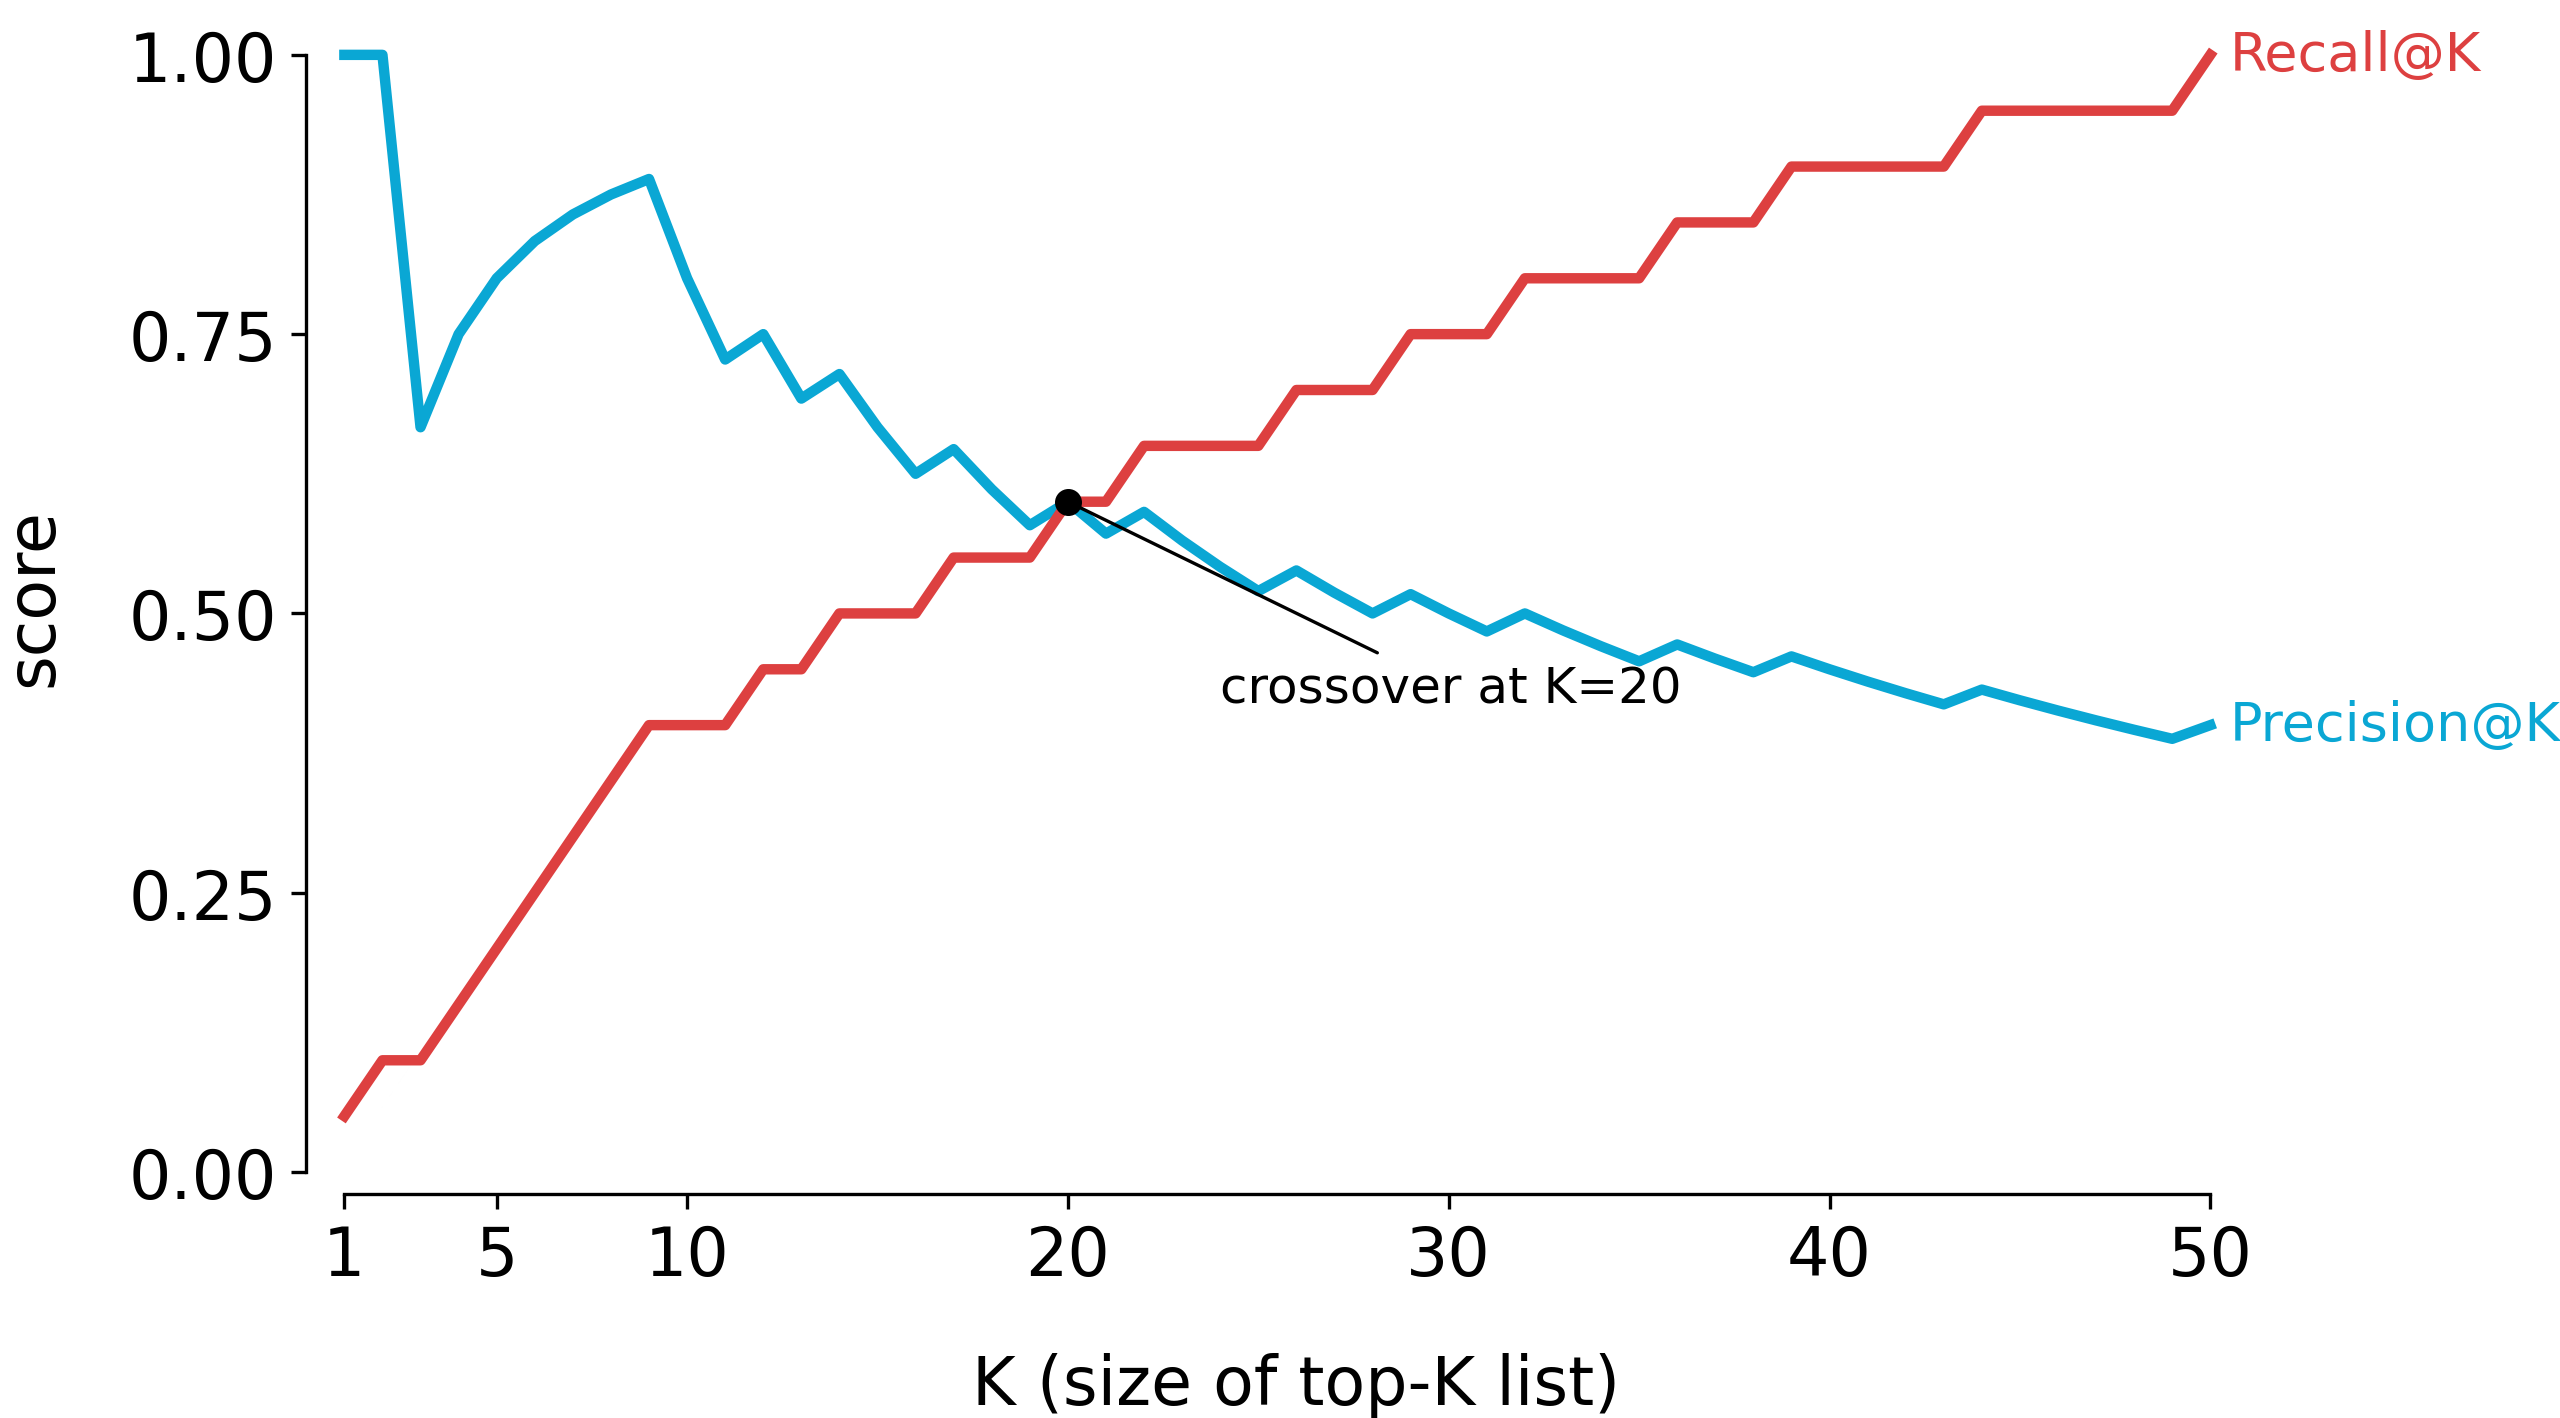
\includegraphics[width=0.85\textwidth]{figures/at_K_precision_recall.png}
\end{figure*}

\textbf{Figure.} Precision@$K$ (blue) falls and Recall@$K$ (red) rises as $K$ grows. The crossover at $K = 20$ is where both curves agree: $60\%$ of relevant items retrieved at $60\%$ precision. Picking $K$ to the left of the crossover means optimizing for a clean top of the list; to the right, for covering more of the relevant set. The shape of the two curves is the practical artifact — the exact crossover shifts with the underlying relevance distribution.

\orangebox{Did you know that...}
{The choice of $K$ is often driven by UI constraints. If a mobile app shows five cards on screen, $Precision@5$ measures exactly the value of that screen. Reporting $Precision@10$ when only five are visible measures a different product than the one users see.}

\textbf{Other related metrics}

Common @K variants include Precision@$K$, Recall@$K$, MAP@$K$, and nDCG@$K$. For a binary check of whether any relevant item appears in the top-$K$, see Hit Rate.

% ---------- Mean Reciprocal Rank ----------
\clearpage
\thispagestyle{rankingstyle}
\section{Mean Reciprocal Rank}
\subsection{MRR}

MRR scores a system on a narrow question: how high in the list is the first relevant result? Average that reciprocal across all queries and the result is MRR. The metric heavily weights the rank-$1$ result and gives little credit when the first relevant item appears at rank $5$ or $10$ — useful for tasks where users abandon the list after the first miss.

\begin{center}
    \tikz{
        \node[inner sep=2pt, font=\Large] (a) {
            {
                $\displaystyle
                MRR = \frac{1}{{\color{nmlred}|Q|}} \sum_{i=1}^{|Q|} \frac{1}{{\color{nmlcyan}rank_i}}
                $
            }
        };
        \draw[overlay,-latex,nmlred, semithick] ($(a.south)+(-0.5,0.2)$) to[bend left=15] node[pos=1, left] {number of queries} +(-1,-.5);
        \draw[overlay,-latex,nmlcyan, semithick] ($(a.north)+(2.0,-0.1)$) to[bend left=15] node[pos=1, right] {first relevant rank} +(1,.5);
    }
\end{center}

MRR lives in $[0, 1]$. A score of $1$ means the relevant item sits at rank $1$ for every query; $0.5$ means the average first-hit is at rank $2$. The decay is hyperbolic — rank $5$ scores $0.2$, rank $20$ scores $0.05$ — so anything past the first relevant item is essentially invisible.

\textbf{When to use MRR?}

Use MRR for known-item search and Q\&A: each query has one canonical answer and the task is to surface it first (``what's the capital of Belgium?''). Avoid MRR when queries have multiple relevant items of comparable value (movies, news) — MRR scores the same whether the slots after the first hit are gold or junk.

\coloredboxes{
    \item Mirrors known-item search. Users want the answer at rank $1$, and MRR penalizes anything below it.
    \item Bounded in $[0, 1]$ and averageable across queries with no normalization.
}
{
    \item Ignores items below the first hit. $[\textit{relevant, junk, junk}]$ and $[\textit{relevant, gold, gold}]$ score the same.
    \item Steep penalty for top-of-list misses. Rank $1$ to rank $2$ halves the score; rank $1$ to rank $10$ drops it by $90\%$.
    \item Inflatable with short rankings — pair MRR with Recall or coverage.
}

\clearpage

\thispagestyle{customstyle}

\begin{figure*}[ht!]
    \centering
    \includegraphics[width=0.6\textwidth]{figures/MRR_reciprocal_rank.png}
\end{figure*}

\textbf{Figure.} Each query contributes the reciprocal of its first-relevant rank to the MRR sum. The drop is fast: rank $1$ gives $1.0$, rank $2$ gives $0.5$, rank $5$ gives $0.2$. Past rank $10$ the reciprocal is small enough that it barely matters whether the relevant item appeared at rank $11$ or rank $1000$ — MRR cares almost exclusively about the top of the list.

\orangebox{Did you know that...}
{MRR is the default scorer for question-answering benchmarks like TREC-QA and Natural Questions because the task is structurally known-item: there is one right answer and the user wants it first. Swapping MRR for nDCG only changes the score on queries with multiple plausible answers — for single-answer queries the two are essentially equivalent.}

\textbf{Other related metrics}

For multi-relevant evaluation use MAP. For graded relevance (some items more relevant than others, e.g., a five-star rating system) use nDCG — it credits every relevant item with a position-discounted contribution, whereas MRR collapses the entire list to a single number from the first hit. For a binary top-$K$ check use Hit Rate.


% ---------- Mean Average Precision ----------
\clearpage
\thispagestyle{rankingstyle}
\section{Mean Average Precision}
\subsection{Mean Average Precision}

MAP rewards rankers for placing relevant items high in the list. For each query, walk down the ranking and average the precision at every position where a relevant item appears — that is the Average Precision (AP). MAP is the mean of AP across queries. A relevant item at rank $1$ contributes precision $1.0$; at rank $10$ it contributes $0.1$, so MAP collapses when relevant items are buried.

\begin{center}
    \tikz{
        \node[inner sep=2pt, font=\Large] (a) {
            {
                $\displaystyle
                MAP = \frac{1}{{\color{nmlred}|Q|}} \sum_{q=1}^{|Q|} \frac{1}{|{\color{nmlcyan}R_q}|} \sum_{k=1}^{n} {\color{nmlpurple}P(k)} \cdot {\color{nmlcyan}rel(k)}
                $
            }
        };
        \draw[overlay,-latex,nmlred, semithick] ($(a.south)+(-1.5,0.2)$) to[bend left=15] node[pos=1, left] {number of queries} +(-1,-.5);
        \draw[overlay,-latex,nmlcyan, semithick] ($(a.north)+(2.0,-0.1)$) to[bend left=15] node[pos=1, right] {relevant items} +(1,.5);
        \draw[overlay,-latex,nmlpurple, semithick] ($(a.south)+(2.5,0.3)$) to[bend left=15] node[pos=1, left] {precision at $k$} +(-1,-.5);
    }
\end{center}

MAP lives in $[0, 1]$. A perfect ranking — every relevant item ahead of every irrelevant one — scores $1$. The gap between MAP and the prevalence baseline (relevant items / list length) measures how much ordering work the model adds on top of plain retrieval.

\textbf{When to use MAP?}

Use MAP when relevance is binary, the full ranked list matters, and you want one number for precision plus order. It is the standard for binary-judgment IR benchmarks. Avoid MAP for graded relevance (use nDCG) or top-only evaluation (use MRR or Precision@$K$) — averaging across all positions lets a strong tail mask a weak top.

\coloredboxes{
    \item Captures precision and rank order in one number. A model that surfaces relevant items earlier always scores higher.
    \item Averages cleanly across queries with different numbers of relevant items — AP is already per-query normalized.
}
{
    \item Assumes binary relevance. No way to say ``item A is more relevant than item B'' the way nDCG can.
    \item Requires complete labels. If a query has five relevant items and only three are labeled, AP is biased downward.
    \item Hard to translate to a user-facing story. ``MAP $= 0.42$'' lands flat next to ``$Precision@10 = 0.6$''.
}

\clearpage
\thispagestyle{customstyle}

\begin{figure*}[ht!]
    \centering
    \includegraphics[width=0.85\textwidth]{figures/MAP_good_vs_bad.png}
\end{figure*}

\textbf{Figure.} Both rankings retrieve four relevant items. The left places them at ranks $1, 2, 3, 6$ and earns $AP = 0.92$; the right at ranks $4, 7, 9, 10$ and earns $AP = 0.32$. Same recall, very different MAP — exactly the gap MAP exists to measure.

\orangebox{Did you know that...}
{MAP became the default scorer for the TREC (Text REtrieval Conference) evaluations, which have been benchmarking information retrieval systems since 1992. The choice was deliberate: MAP credits precision at every position where a relevant item appears, so a system that surfaces the same items earlier always wins — exactly the property TREC wanted to reward across thirty years of system comparisons.}

\textbf{Other related metrics}

For graded relevance use nDCG. For top-only evaluation use MRR or Precision@$K$. AP and MAP are related as point and average: AP is the per-query score, MAP is the mean across queries.

% good resources for inpiration for visual: https://juneandrews.com/2014/12/15/mean-average-precision-isnt-so-nice/
% https://sdsawtelle.github.io/blog/output/mean-average-precision-MAP-for-recommender-systems.html

% ---------- Hit Rate ----------
\clearpage
\thispagestyle{rankingstyle}
\section{Hit Rate}
\subsection{Hit Rate}

Hit Rate answers a yes-no question per user: did the top-$K$ list contain at least one relevant item? Average that indicator across users and you have the Hit Rate of the system. It ignores how many relevant items appeared and where they were — only whether the user got something or nothing.

\begin{center}
    \tikz{
        \node[inner sep=2pt, font=\Large] (a) {
            {
                $\displaystyle
                Hit\ Rate = \frac{1}{{\color{nmlred}|U|}} \sum_{u=1}^{|U|} {\color{nmlgreen}\mathds{1}}\left(|{\color{nmlcyan}R_u} \cap {\color{nmlpurple}Top\text{-}K_u}| > 0\right)
                $
            }
        };
        \draw[overlay,-latex,nmlred, semithick] ($(a.south)+(-2.0,0.2)$) to[bend left=15] node[pos=1, left] {number of users} +(-1,-.5);
        \draw[overlay,-latex,nmlcyan, semithick] ($(a.north)+(2.0,-0.1)$) to[bend right=15] node[pos=1, left] {relevant items} +(-1,.5);
        \draw[overlay,-latex,nmlpurple, semithick] ($(a.north)+(3.5,-0.1)$) to[bend left=15] node[pos=1, right] {top-K items} +(1,.5);
    }
\end{center}

A Hit Rate of $0.72$ means $72\%$ of users got at least one relevant item in their top-$K$ list; the other $28\%$ saw nothing useful. The low bar makes Hit Rate the right metric for catching a specific failure: lists that look diverse but happen to miss every user's actual interests.

\textbf{When to use Hit Rate?}

Use Hit Rate as a floor for top-$K$ quality: ``what fraction of sessions show at least one relevant item?'' translates directly to product metrics. Avoid Hit Rate as the primary optimization target — a model can score well by recommending broadly, with no signal about whether the hit is buried in junk.

\coloredboxes{
    \item Easy to communicate. ``$72\%$ of sessions see at least one relevant item'' maps directly onto product metrics like activation or session quality.
    \item Robust to sparsity and missing labels. A single relevant item per user is enough to score.
    \item Endpoint-interpretable. $0$ means total failure; $1$ means every user is served.
}
{
    \item Position-blind. A relevant item at rank $1$ scores the same as one at rank $K$.
    \item Count-blind. A list with one relevant item scores the same as a list with five.
    \item Saturates fast. At small $K$ the metric undercounts; at large $K$ it pins to $1$. Pick $K$ where Hit Rate still moves between models.
}

\clearpage
\thispagestyle{customstyle}

\begin{figure*}[ht!]
    \centering
    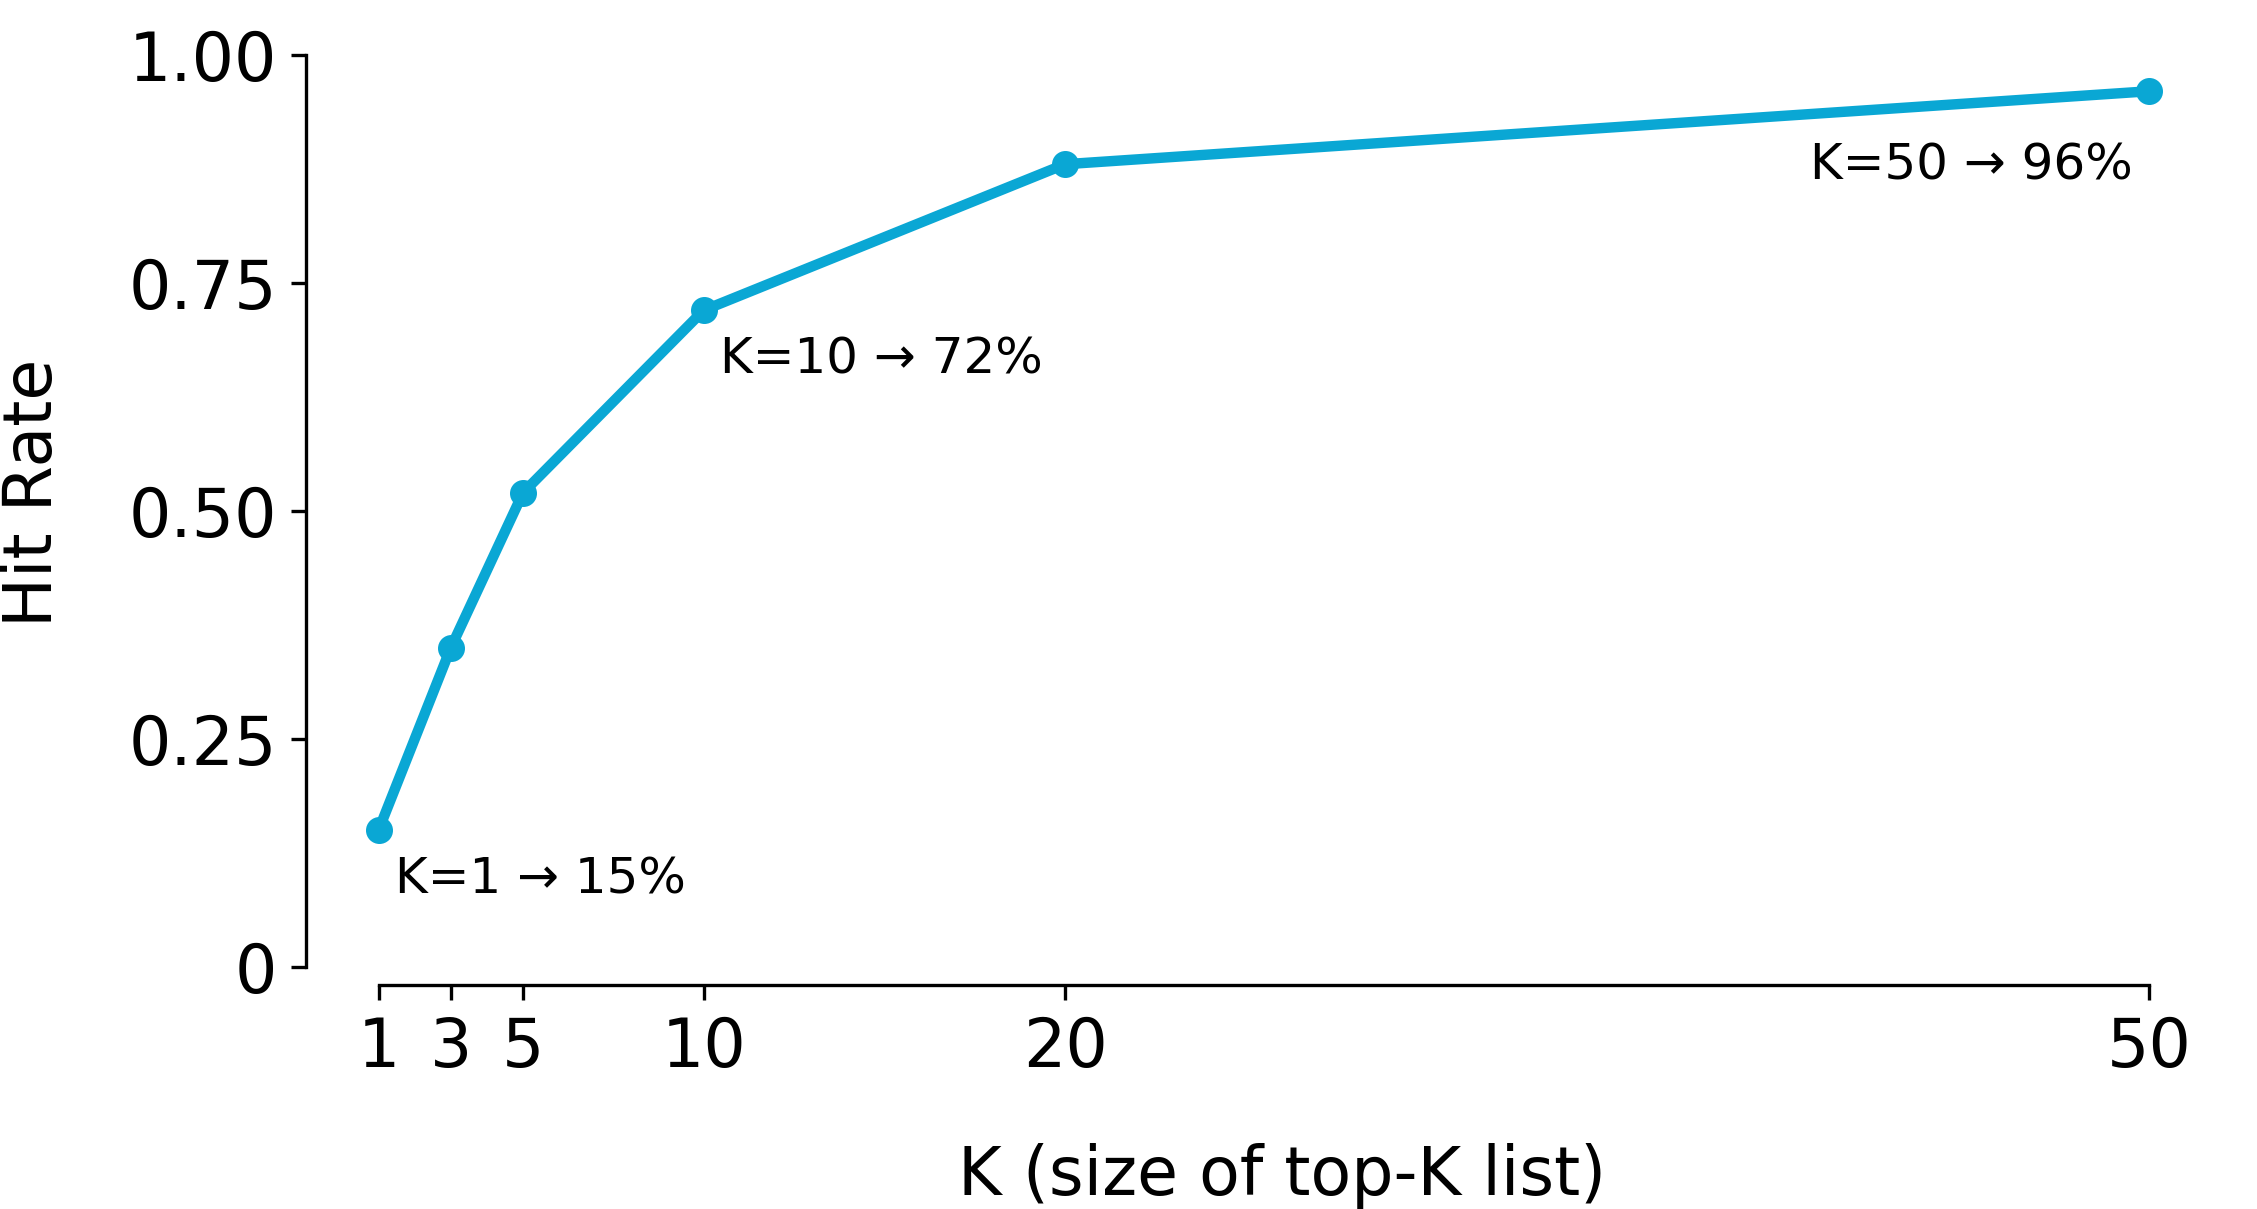
\includegraphics[width=0.6\textwidth]{figures/Hit_Rate_vs_K.png}
\end{figure*}

\textbf{Figure.} Hit Rate climbs with $K$: at $K = 1$ only $15\%$ of users see a relevant item in the first slot; at $K = 50$ that rises to $96\%$. The curve flattens as $K$ grows because the remaining failures are users with no relevant items anywhere in the top-$50$ — stretching $K$ further does not help that segment.

\orangebox{Did you know that...}
{Recommender systems papers often call Hit Rate ``Recall@$K$'' and use the two interchangeably. They are the same metric only when each user has exactly one relevant item — the typical leave-one-out evaluation setup. With multiple relevant items per user, Recall@$K$ measures the fraction retrieved, while Hit Rate stays binary. The naming clash trips up cross-paper comparisons more often than you would expect.}

\textbf{Other related metrics}

For position-aware evaluation use MRR or nDCG. For counting how many relevant items the list retrieved, use Recall@$K$. Hit Rate is the binary collapse of Recall@$K$.

% ---------- Cumulative Gain ----------
\clearpage
\thispagestyle{rankingstyle}
\section{CG}
\subsection{Cumulative Gain}

Cumulative Gain (CG) sums the relevance scores of the items in a recommendation list. With graded relevance — $3$ for ``perfect'', $1$ for ``marginal'', $0$ for ``irrelevant'' — $CG_K$ is the total relevance packed into the top-$K$. The catch is that CG ignores rank: a relevant item at position $1$ adds the same as one at position $K$.

\begin{center}
    \tikz{
        \node[inner sep=2pt, font=\Large] (a) {
            {
                $\displaystyle
                CG_p = \sum_{i=1}^{{\color{nmlred}p}} {\color{nmlcyan}rel_i}
                $
            }
        };
        \draw[overlay,-latex,nmlred, semithick] ($(a.north)+(0.8,-0.1)$) to[bend left=15] node[pos=1, right] {number of items} +(1,.5);
        \draw[overlay,-latex,nmlcyan, semithick] ($(a.south)+(1.2,0.2)$) to[bend left=15] node[pos=1, left] {relevance of item $i$} +(-1,-.5);
    }
\end{center}

CG is unbounded and order-invariant: two lists with the same items in different orders have identical CG. That makes it useful as a baseline number — ``how much total relevance did we retrieve?'' — but not as a standalone ranking metric. DCG and nDCG (next pages) fix the rank-insensitivity by discounting later positions.

\textbf{When to use CG?}

Use CG when only total retrieved relevance matters and ordering is decided downstream (a re-ranker reshuffles the list, or items are shown simultaneously). Avoid CG when position matters to the user — which covers most ranking applications. Use DCG or nDCG instead.

\coloredboxes{
    \item Simplest relevance aggregation possible: add up the scores. Trivial to compute and explain.
    \item Works with graded relevance out of the box, unlike Hit Rate or binary $Precision@K$.
}
{
    \item Order-invariant. A list with the best item at rank $1$ scores the same as one with the best item at rank $K$.
    \item Not normalized. $CG = 12$ vs $CG = 6$ across queries says nothing about which ranking was better.
    \item Falls back to a raw count of relevant items when only binary labels are available.
}

\clearpage
\thispagestyle{customstyle}

\begin{figure*}[ht!]
    \centering
    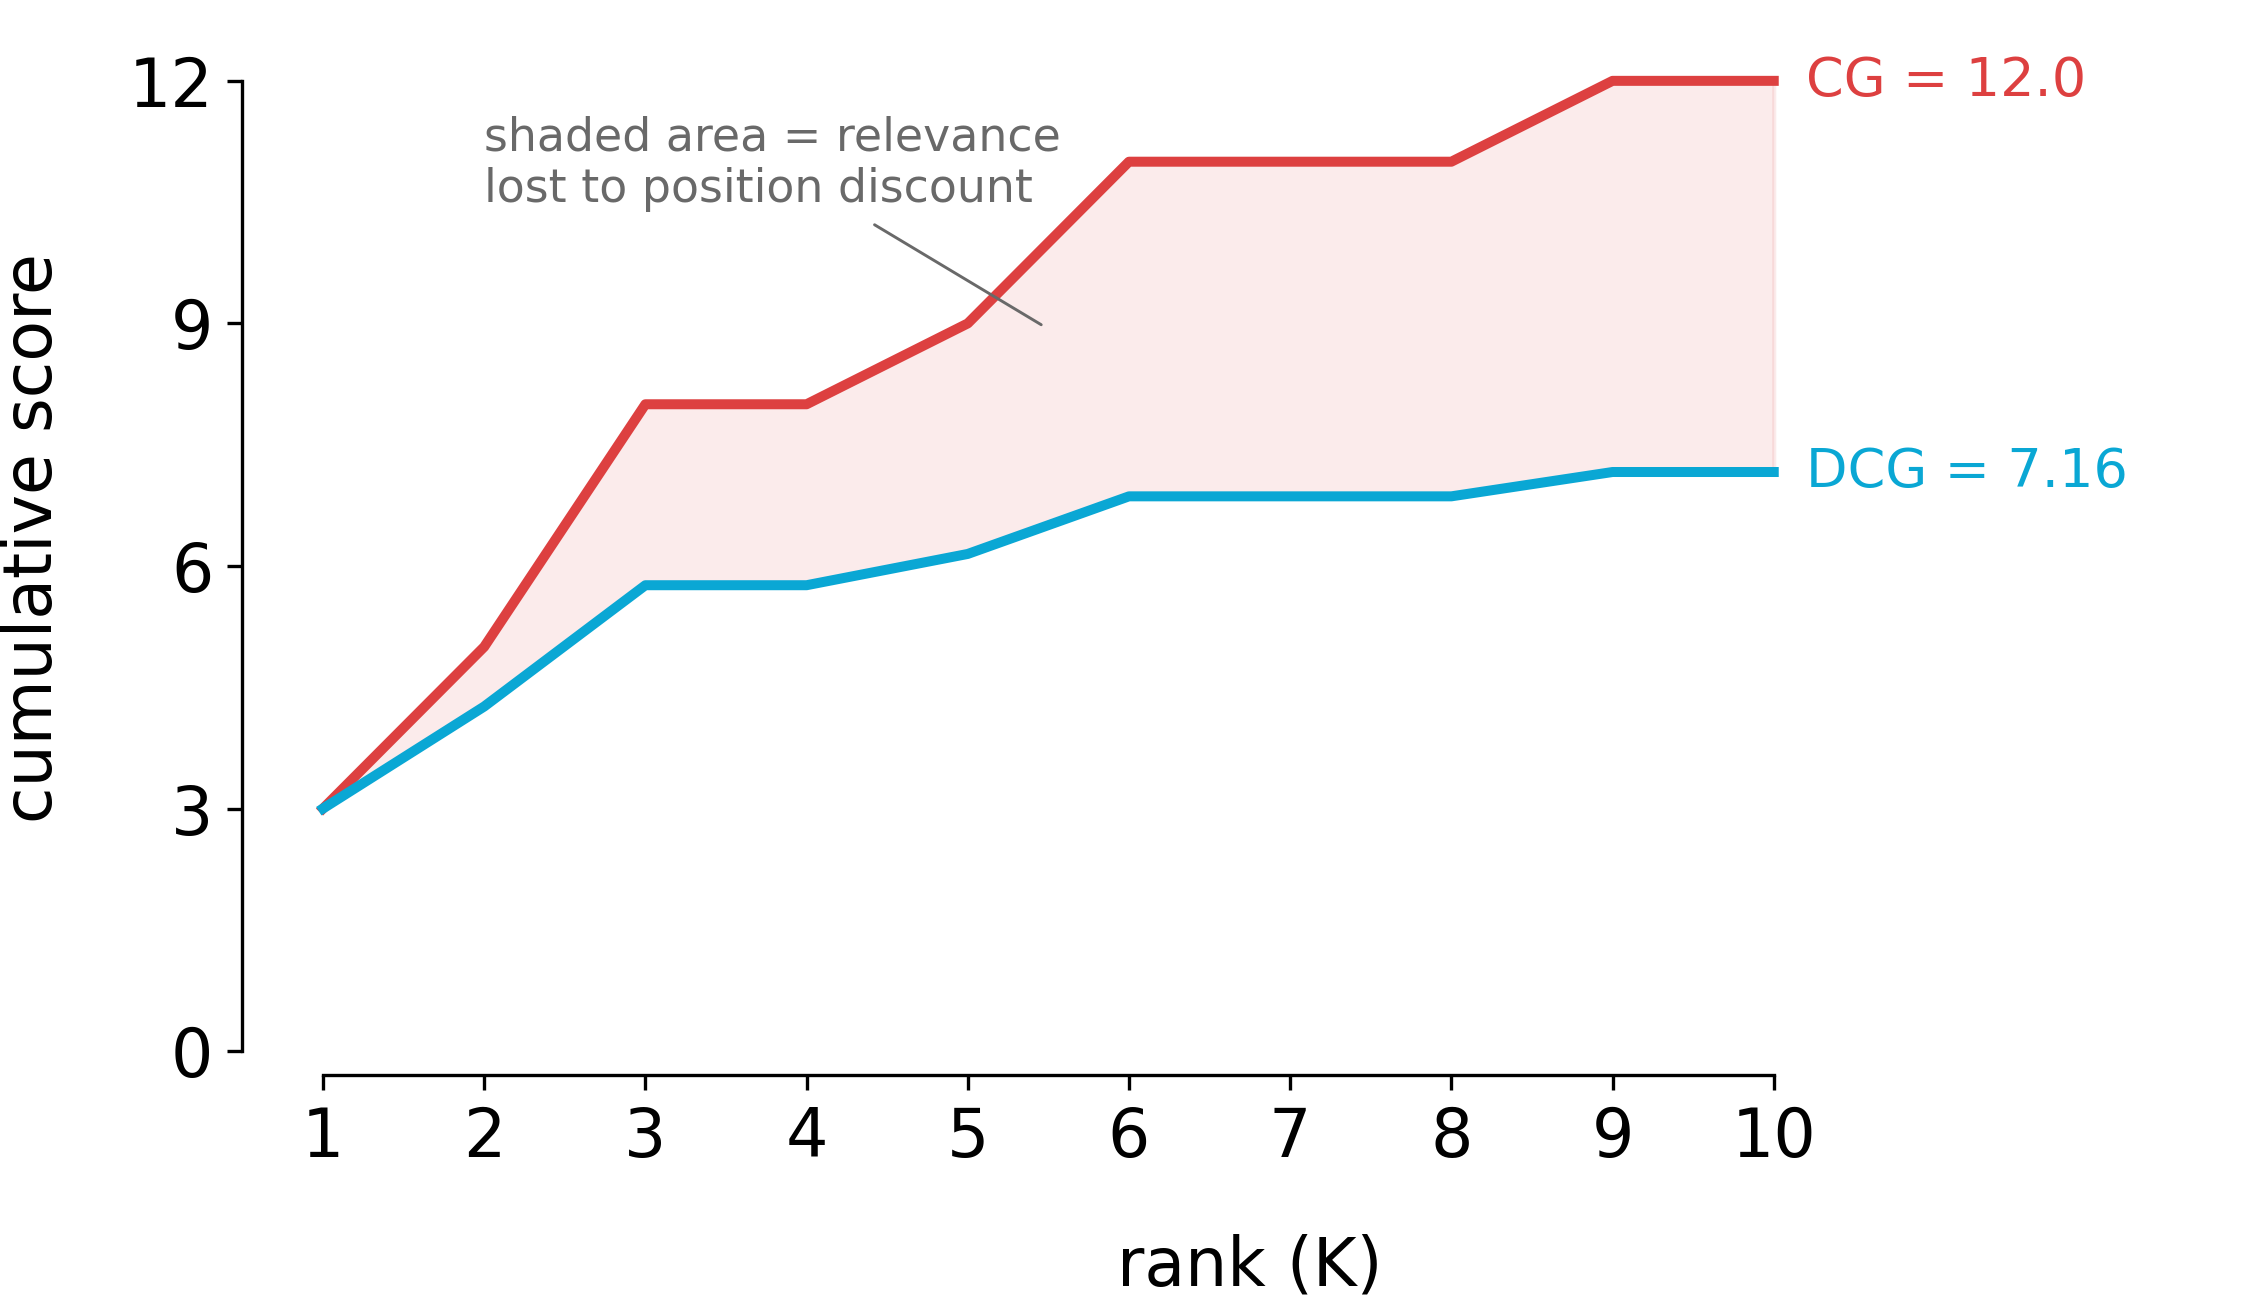
\includegraphics[width=0.6\textwidth]{figures/CG_vs_DCG.png}
\end{figure*}

\textbf{Figure.} CG (red) and DCG (blue) start at the same point — the first item contributes its full relevance to both. As $K$ grows, DCG falls behind because every position past rank $1$ takes a logarithmic discount, while CG keeps treating every position equally. The widening gap is the cost of ignoring position.

\orangebox{Did you know that...}
{The order-invariance of CG is its entire design flaw: swap any two items and the score is unchanged, which makes CG useless for ranking. The metric still gets used in retrieval-then-rerank pipelines, where the retrieval stage scores raw recall and a downstream model handles the ordering. Outside that pattern, CG on its own in a results table is a red flag.}

\textbf{Other related metrics}

DCG extends CG by discounting later positions. nDCG normalizes DCG against the ideal ranking, so scores are comparable across queries with different relevance budgets. In practice, CG is the warm-up step toward those two.

% ---------- Discounted Cumulative Gain ----------
\clearpage
\thispagestyle{rankingstyle}
\section{DCG}
\subsection{Discounted Cumulative Gain}

Discounted Cumulative Gain (DCG) improves upon CG by introducing a position-based discounting factor.
It accounts for the fact that relevant items appearing earlier in the list are more valuable than those appearing later.

\begin{center}
    \tikz{
        \node[inner sep=2pt, font=\Large] (a) {
            {
                $\displaystyle
                DCG_p = \sum_{i=1}^{{\color{nmlred}p}} \frac{{\color{nmlcyan}rel_i}}{{\color{nmlpurple}\log_2(i + 1)}}
                $
            }
        };
        \draw[overlay,-latex,nmlcyan, semithick] ($(a.north)+(1.0,-0.1)$) to[bend right=15] node[pos=1, left] {relevance of item $i$} +(-1,.5);
        \draw[overlay,-latex,nmlpurple, semithick] ($(a.south)+(1.5,0.3)$) to[bend left=15] node[pos=1, left] {position discount} +(-1,-.5);
    }
\end{center}

This logarithmic discounting ensures that higher-ranked relevant items contribute more to the score.

\textbf{When to use DCG?}

Use DCG when you want to measure both the total relevance and the order of relevant items in a ranked list. It is particularly
useful for search engines, recommendation systems, and ranking models where placing relevant items at the top is crucial.

\coloredboxes{
    \item Accounts for ranking order. Relevant items appearing earlier in the list are weighted more heavily.
    \item More realistic than CG. Since users are more likely to engage with items at the top, DCG better reflects
    real-world relevance.
}
{
    \item Not normalized — DCG values depend on the number and relevance of items, making cross-query comparison difficult.
    \item Human data labelers must provide relevance scores to compute the total accumulated relevance.
}

\clearpage
\thispagestyle{customstyle}

\begin{figure*}[ht!]
    \centering
    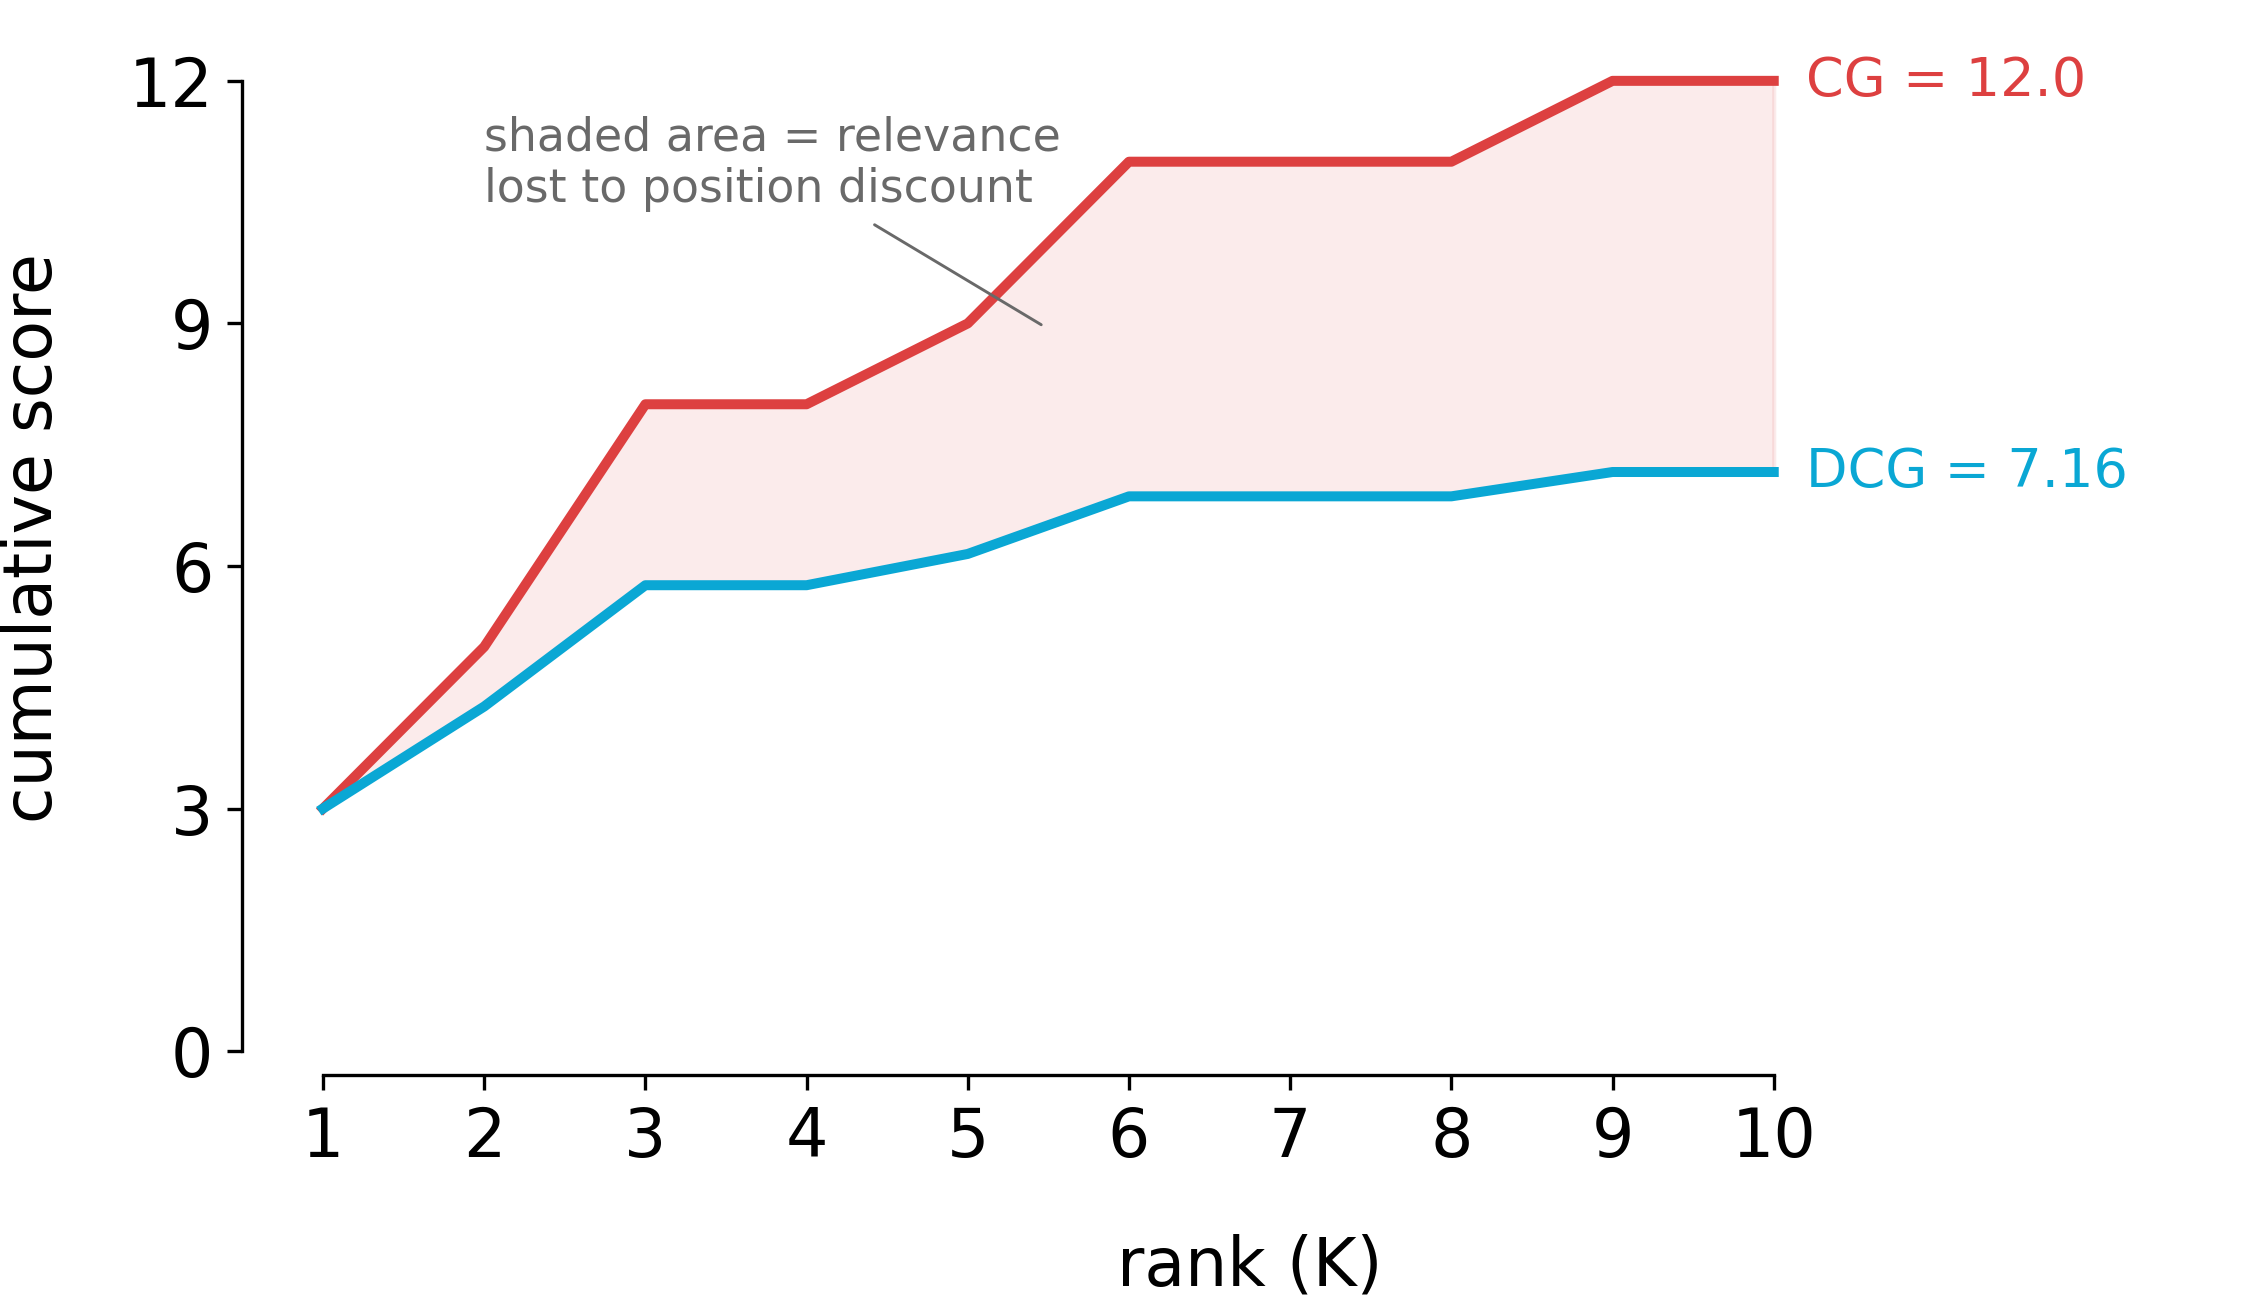
\includegraphics[width=0.6\textwidth]{figures/CG_vs_DCG.png}
\end{figure*}

\textbf{Figure.} DCG (blue) applies logarithmic discounting, giving more weight to items ranked higher. CG (red) treats all positions equally, making DCG a more realistic measure.

\orangebox{Did you know that...}
{The logarithmic discount in DCG was introduced by J\"{a}rvelin and Kek\"{a}l\"{a}inen in 2002. The choice of $\log_2$ is conventional but arbitrary — some implementations use natural log or $\log_{10}$.}

\textbf{Other related metrics}

DCG builds on CG by adding position discounting. For a normalized version that enables cross-query comparison, use nDCG.
For binary relevance, MAP may be a simpler alternative.

% ---------- Normalized Discounted Cumulative Gain ----------
\clearpage
\thispagestyle{rankingstyle}
\section{nDCG}
\subsection{Normalized Discounted Cumulative Gain}

Normalized Discounted Cumulative Gain (nDCG) extends DCG by normalizing it relative to the Ideal Discounted Cumulative Gain
(IDCG)—the best possible ranking of the same set of items. This ensures that scores are comparable across different users
and queries.

\begin{center}
    \tikz{
        \node[inner sep=2pt, font=\Large] (a) {
            {
                $\displaystyle
                nDCG_p = \frac{{\color{nmlcyan}DCG_p}}{{\color{nmlpurple}IDCG_p}}
                $
            }
        };
        \draw[overlay,-latex,nmlcyan, semithick] ($(a.north)+(0.8,-0.1)$) to[bend right=15] node[pos=1, left] {actual DCG} +(-1,.5);
        \draw[overlay,-latex,nmlpurple, semithick] ($(a.south)+(1.0,0.2)$) to[bend left=15] node[pos=1, left] {ideal DCG} +(-1,-.5);
    }
\end{center}

IDCG is the DCG computed with an optimally ranked list. nDCG values range from 0 to 1, with 1 indicating a perfect ranking.

\textbf{When to use nDCG?}

Use nDCG when you need a standardized ranking metric that allows comparison across different recommendation tasks.
It is widely used in search engines, recommender systems, and ranking models where ranking quality is essential.

\coloredboxes{
    \item Scale-independent. Since it is normalized, NDCG values are comparable across different datasets and users.
    \item Captures both relevance and ranking order. It rewards placing highly relevant items early in the list while
    penalizing poorly ranked relevant items.
}
{
    \item Human data labelers must provide relevance scores to compute the total accumulated relevance.
    \item Not ideal for binary relevance. nDCG is designed for graded relevance; for binary relevance, MAP may be more appropriate.
}

\clearpage
\thispagestyle{customstyle}

\begin{figure*}[ht!]
    \centering
    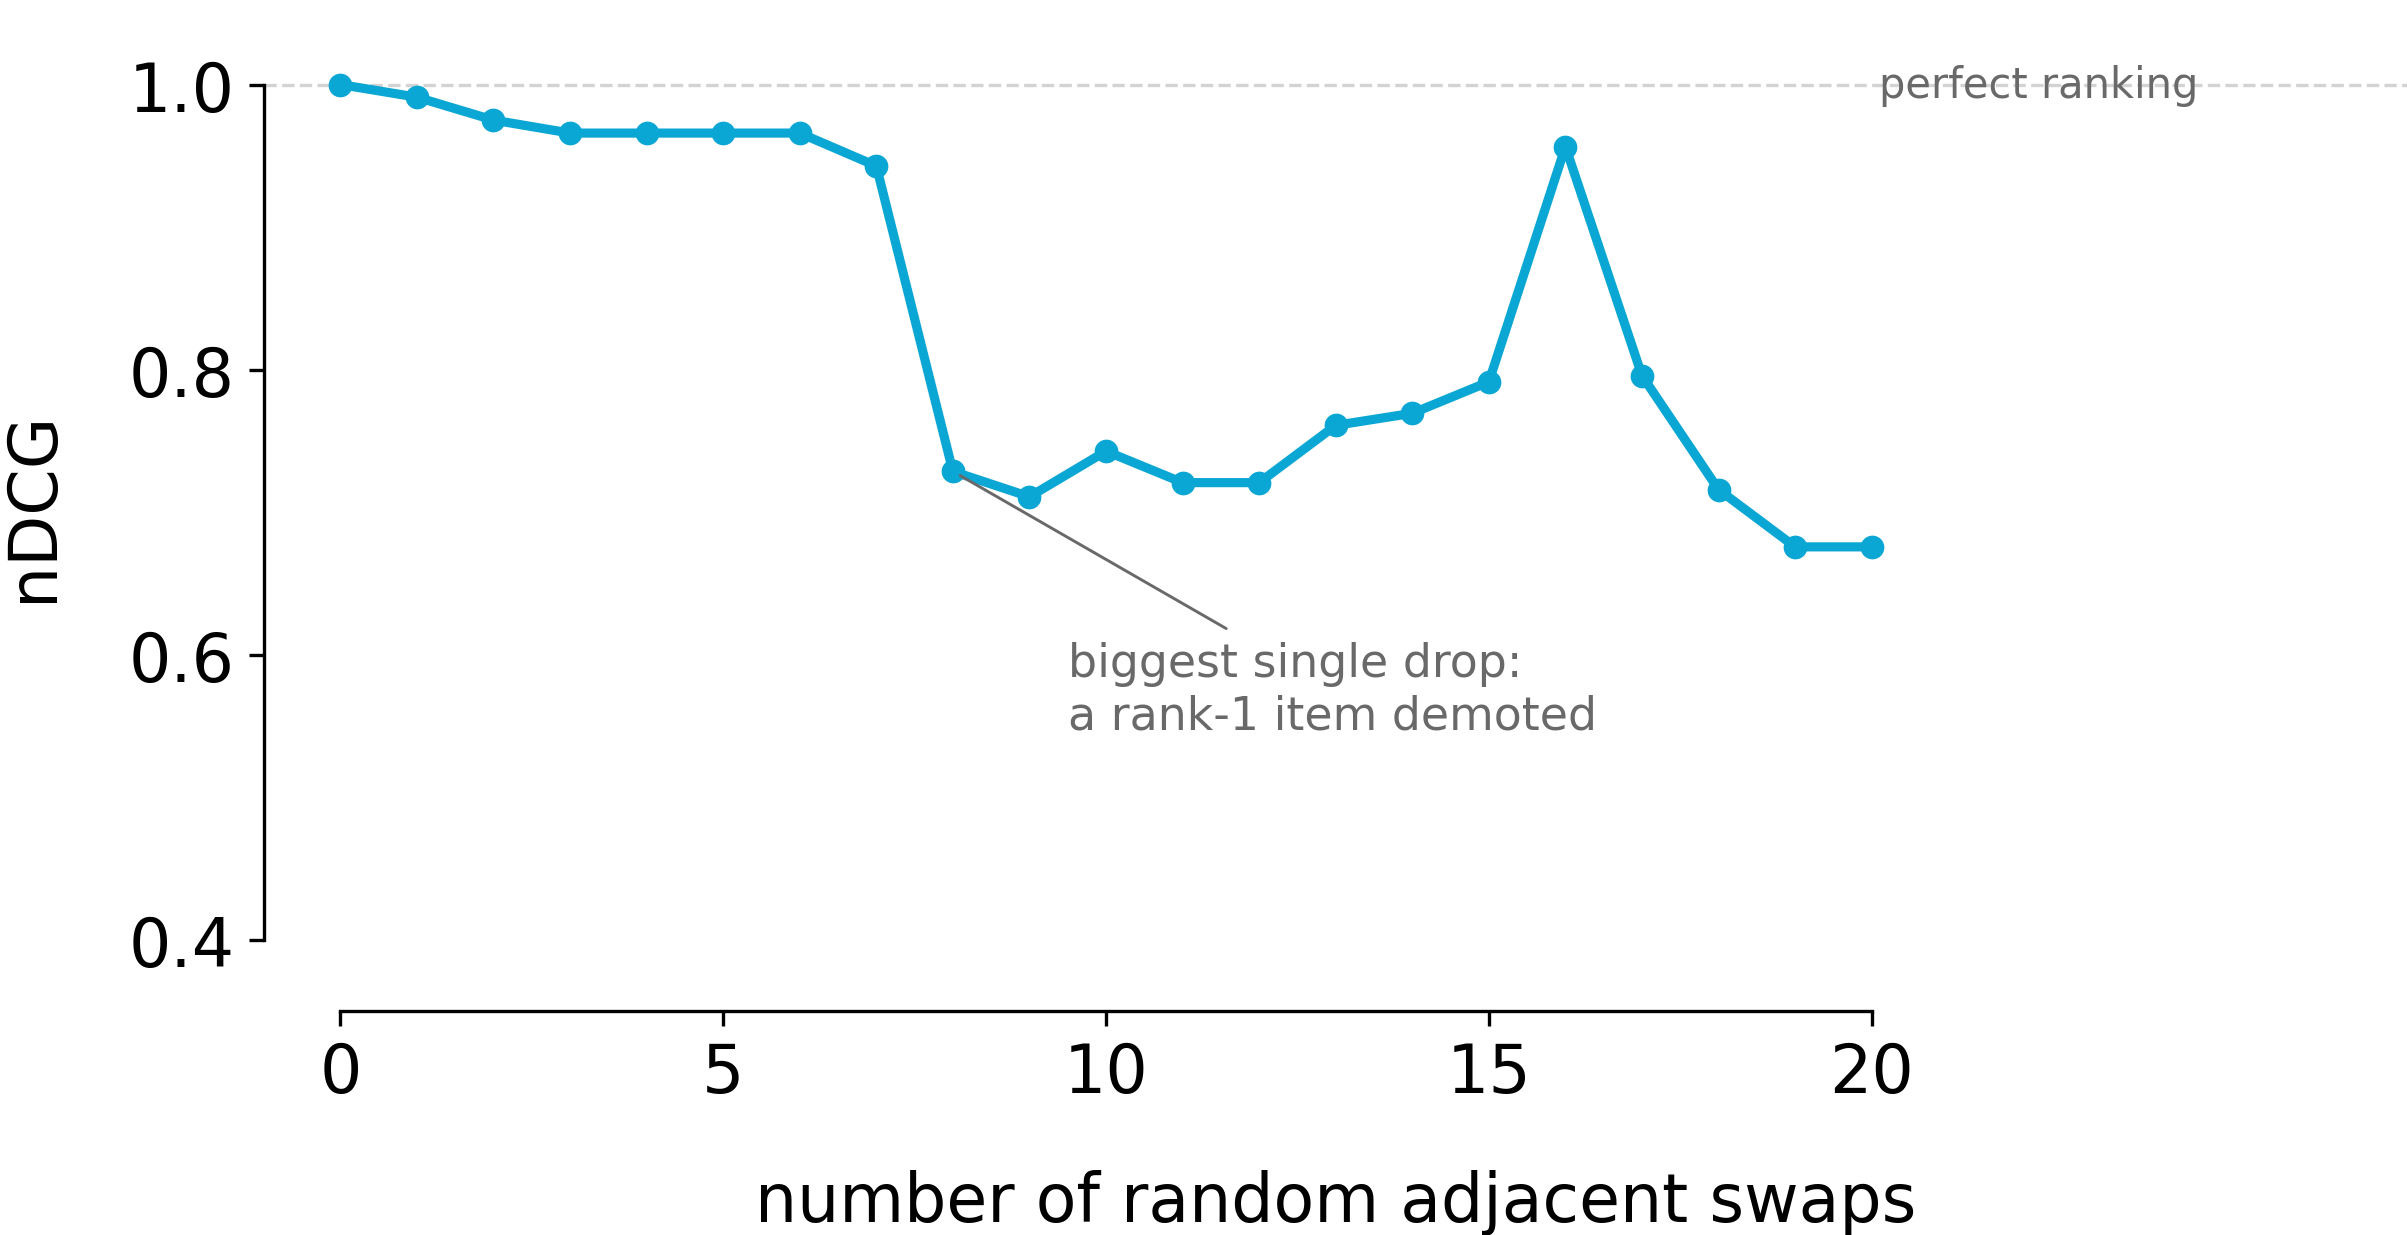
\includegraphics[width=0.6\textwidth]{figures/nDCG_degradation.png}
\end{figure*}

\textbf{Figure.} nDCG decreases as we progressively degrade the ranking by random swaps. A perfect ranking scores 1.0; each swap moves relevant items away from their ideal positions.

\orangebox{Did you know that...}
{nDCG is the standard offline evaluation metric at most major tech companies for search and recommendation systems. It is also the primary metric
used in the annual TREC Web Track and in Kaggle recommendation competitions.}

\textbf{Other related metrics}

nDCG is the normalized version of DCG. For binary relevance scenarios, consider MAP. For evaluating only the first relevant result, use MRR.

% great resource: https://aman.ai/recsys/metrics/#normalized-discounted-cumulative-gain-ndcg-1


% ---------- Fraction of Concordant Pairs ----------
\clearpage
\thispagestyle{rankingstyle}
\section{FCP}
\subsection{Fraction of Concordant Pairs}

Fraction of Concordant Pairs (FCP) is a ranking metric used in recommender systems to evaluate how well a model ranks
preferred items higher than less preferred ones. It measures the proportion of correctly ordered item pairs among all
comparable pairs in a recommendation list. Given a user’s interactions, FCP checks whether the model ranks a more relevant
item above a less relevant one.

\begin{center}
    \tikz{
        \node[inner sep=2pt, font=\Large] (a) {
            {
                $\displaystyle
                FCP = \frac{|{\color{nmlcyan}\text{concordant pairs}}|}{|{\color{nmlpurple}\text{comparable pairs}}|}
                $
            }
        };
        \draw[overlay,-latex,nmlcyan, semithick] ($(a.north)+(0.5,-0.1)$) to[bend right=15] node[pos=1, left] {correctly ordered pairs} +(-1,.5);
        \draw[overlay,-latex,nmlpurple, semithick] ($(a.south)+(1.0,0.3)$) to[bend left=15] node[pos=1, left] {total comparable pairs} +(-1,-.5);
    }
\end{center}

A concordant pair is one where the model correctly ranks a preferred item above a less preferred one. FCP values range from
0 to 1, with 1 indicating a perfect ranking and 0 meaning the model fails to rank preferred items higher.

\textbf{When to use FCP?}

Use FCP when evaluating recommender systems that generate personalized rankings, especially in cases where relative
ranking quality is more important than absolute scores. It is particularly useful in implicit feedback scenarios,
such as e-commerce or media streaming, where explicit relevance scores are unavailable, and user preferences must be
inferred from interactions.

\coloredboxes{
    \item It directly measures how accurately the system's rankings align with user preferences.
}
{
    \item It only evaluates pairs of items where user preferences can be inferred, potentially reducing
    the number of evaluated pairs.
    \item Calculating FCP can be resource-intensive for large datasets, as the number of item pairs grows
    quadratically with dataset size.
}

\clearpage
\thispagestyle{customstyle}

\begin{figure*}[ht!]
    \centering
    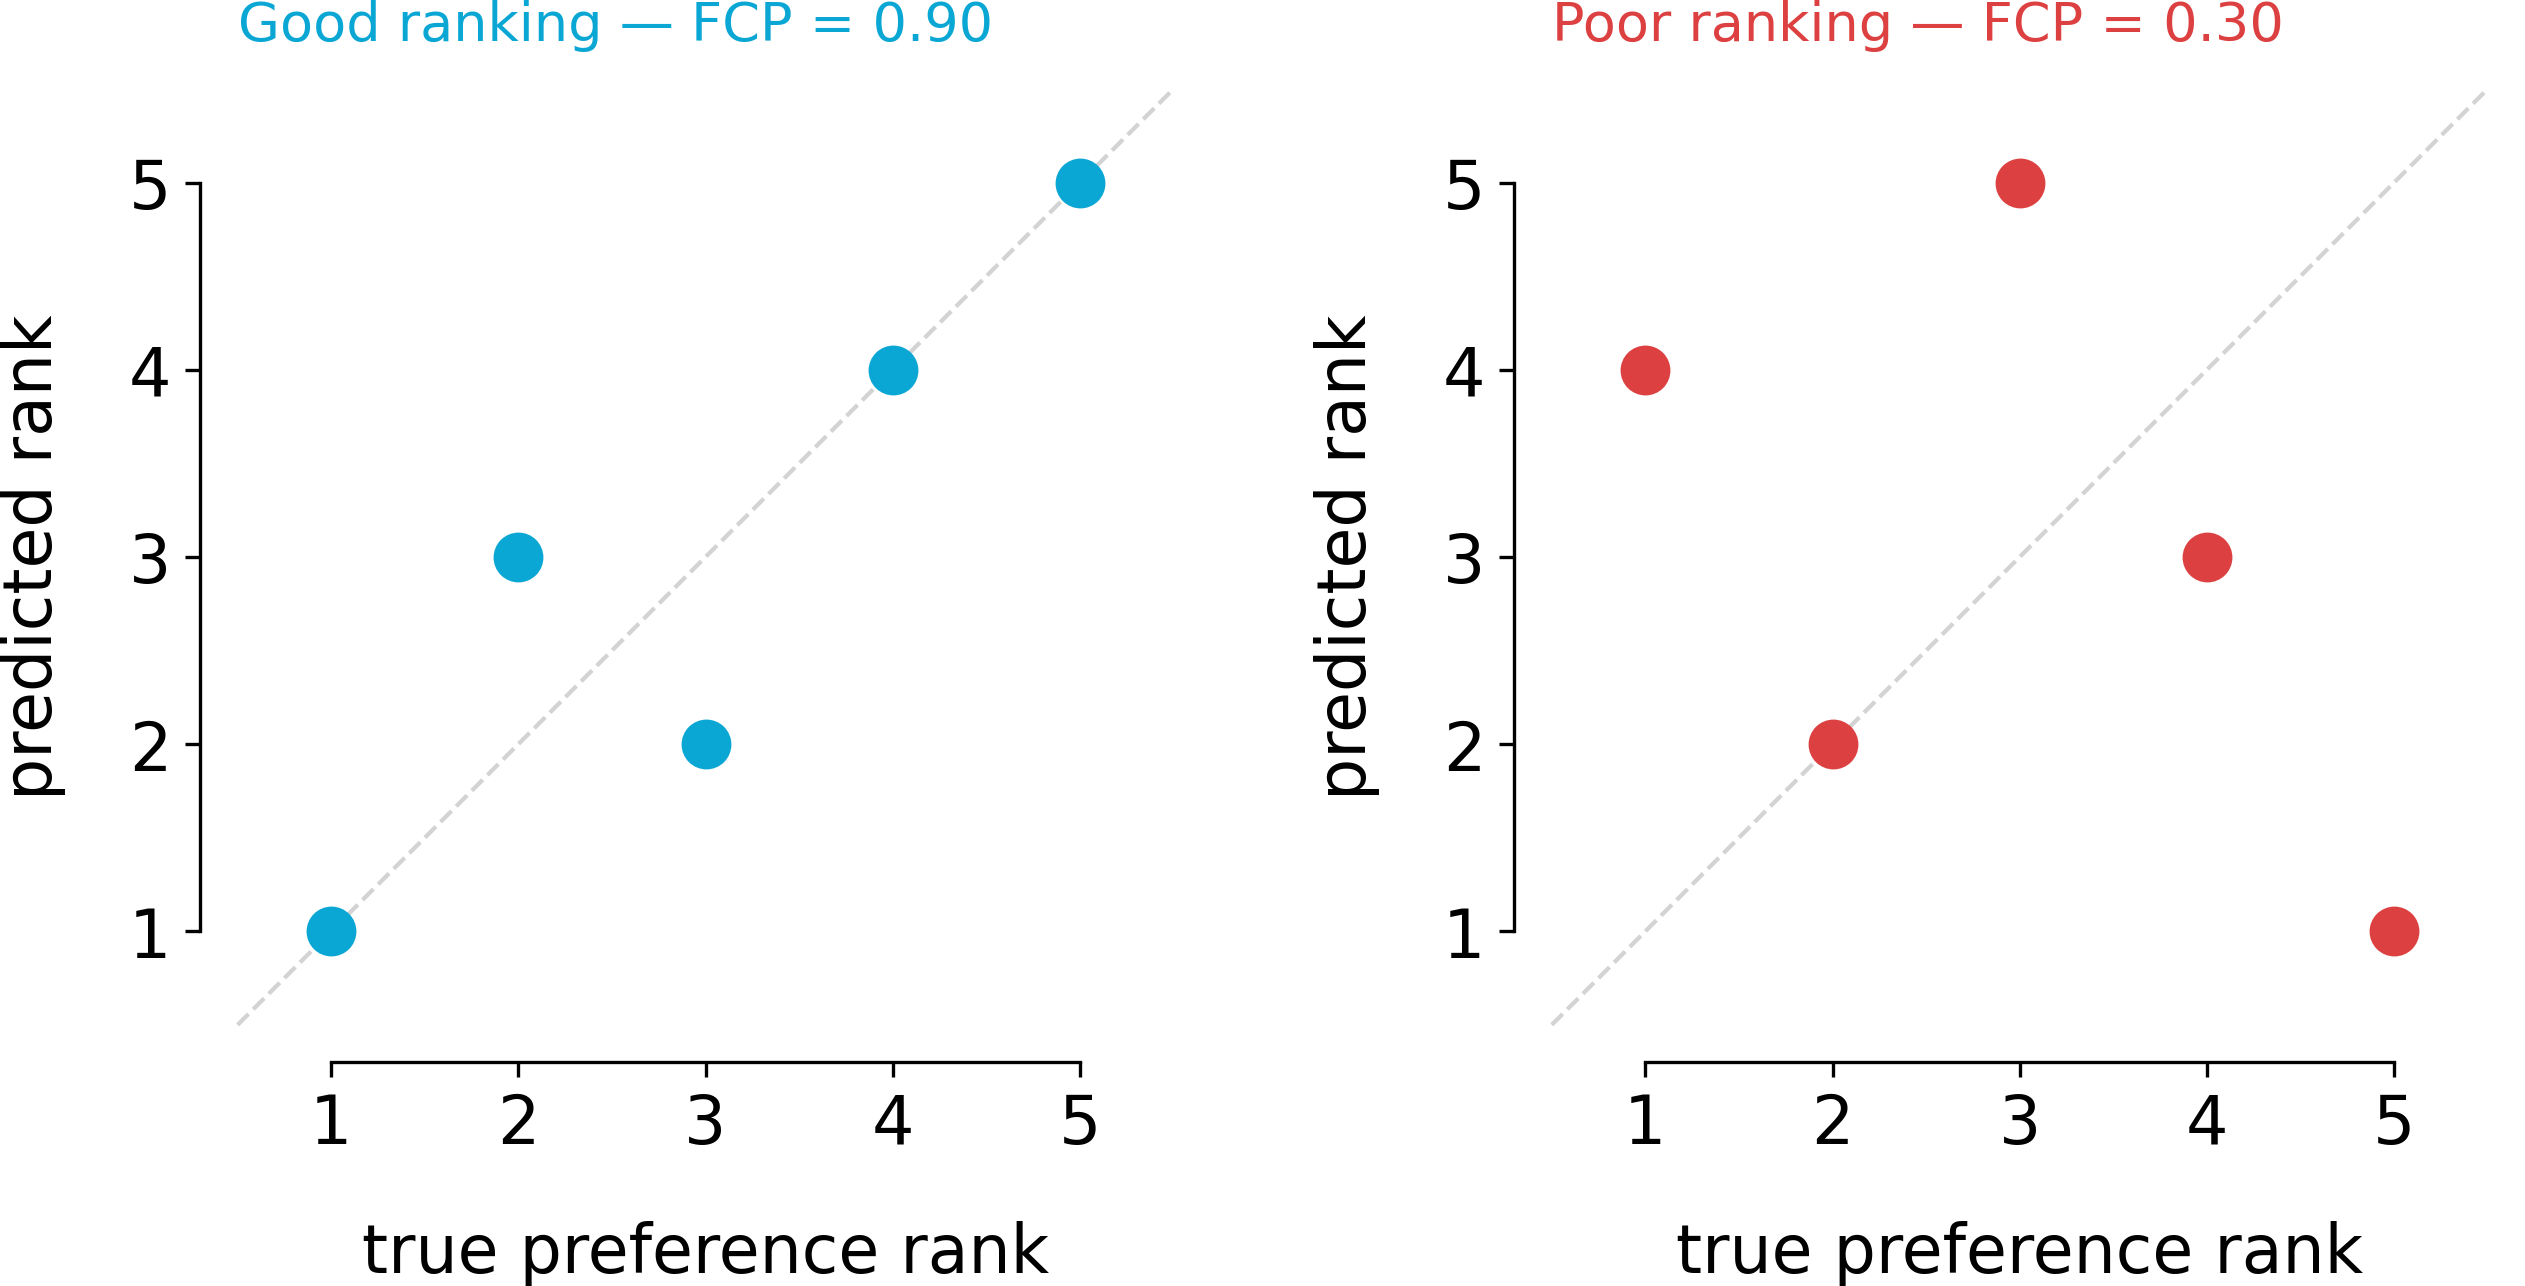
\includegraphics[width=\textwidth]{figures/FCP_comparison.png}
\end{figure*}

\textbf{Figure.} A good ranking (left, FCP=0.90) shows predicted ranks closely matching true preferences. A poor ranking (right, FCP=0.20) shows little agreement.

\orangebox{Did you know that...}
{FCP is closely related to Kendall's tau rank correlation coefficient. Both measure pairwise agreement in rankings, but FCP is expressed as a proportion
while Kendall's tau is normalized to [-1, 1].}

\textbf{Other related metrics}

FCP is a pairwise ranking metric similar to Kendall's tau and Spearman's rank correlation.
For position-weighted evaluation, use nDCG or MAP instead.

% great references: https://aman.ai/recsys/metrics/#fraction-of-concordant-pairs-fcp
% https://www.ijcai.org/Proceedings/13/Papers/449.pdf

% ---------- Diversity ----------
\clearpage
\thispagestyle{rankingstyle}
\section{Diversity}
\subsection{Diversity}

Diversity is a ranking metric used in recommender systems to measure how varied the recommended items are within a given list.
A diverse recommendation set ensures that users are exposed to different categories, genres, or types of content, rather than
receiving highly similar items. This helps prevent redundancy and enhances user discovery. Diversity is often calculated using
pairwise dissimilarity between recommended items.

\begin{center}
    \tikz{
        \node[inner sep=2pt, font=\Large] (a) {
            {
                $\displaystyle
                Diversity = \frac{1}{{\color{nmlred}|L|(|L|-1)}} \sum_{i \in L} \sum_{j \in L, j \neq i} {\color{nmlcyan}d(i, j)}
                $
            }
        };
        \draw[overlay,-latex,nmlred, semithick] ($(a.south)+(-1.5,0.2)$) to[bend left=15] node[pos=1, left] {list size} +(-1,-.5);
        \draw[overlay,-latex,nmlcyan, semithick] ($(a.north)+(3.0,-0.1)$) to[bend left=15] node[pos=1, right] {pairwise dissimilarity} +(1,.5);
    }
\end{center}

A higher Diversity score indicates that the recommended items are more distinct from one another, whereas a lower score
suggests redundancy.

\textbf{When to use Diversity?}

Diversity is particularly important when you want to improve user engagement by introducing varied recommendations. Or when
you want to avoid excessive similarity in recommendations.

\coloredboxes{
    \item Encourages exploration. Users are exposed to a broader range of content, which can increase
    engagement and retention.
    \item Supports long-tail recommendations. Helps surface less popular items that may still be relevant,
    avoiding over-recommendation of mainstream content.
}
{
    \item Potential trade-off with relevance. Increasing diversity may sometimes lead to less relevant recommendations
    for the user.
    \item Hard to define optimal diversity. Too much diversity can lead to recommendations that feel random or disconnected.
}

\clearpage
\thispagestyle{customstyle}

\begin{figure*}[ht!]
    \centering
    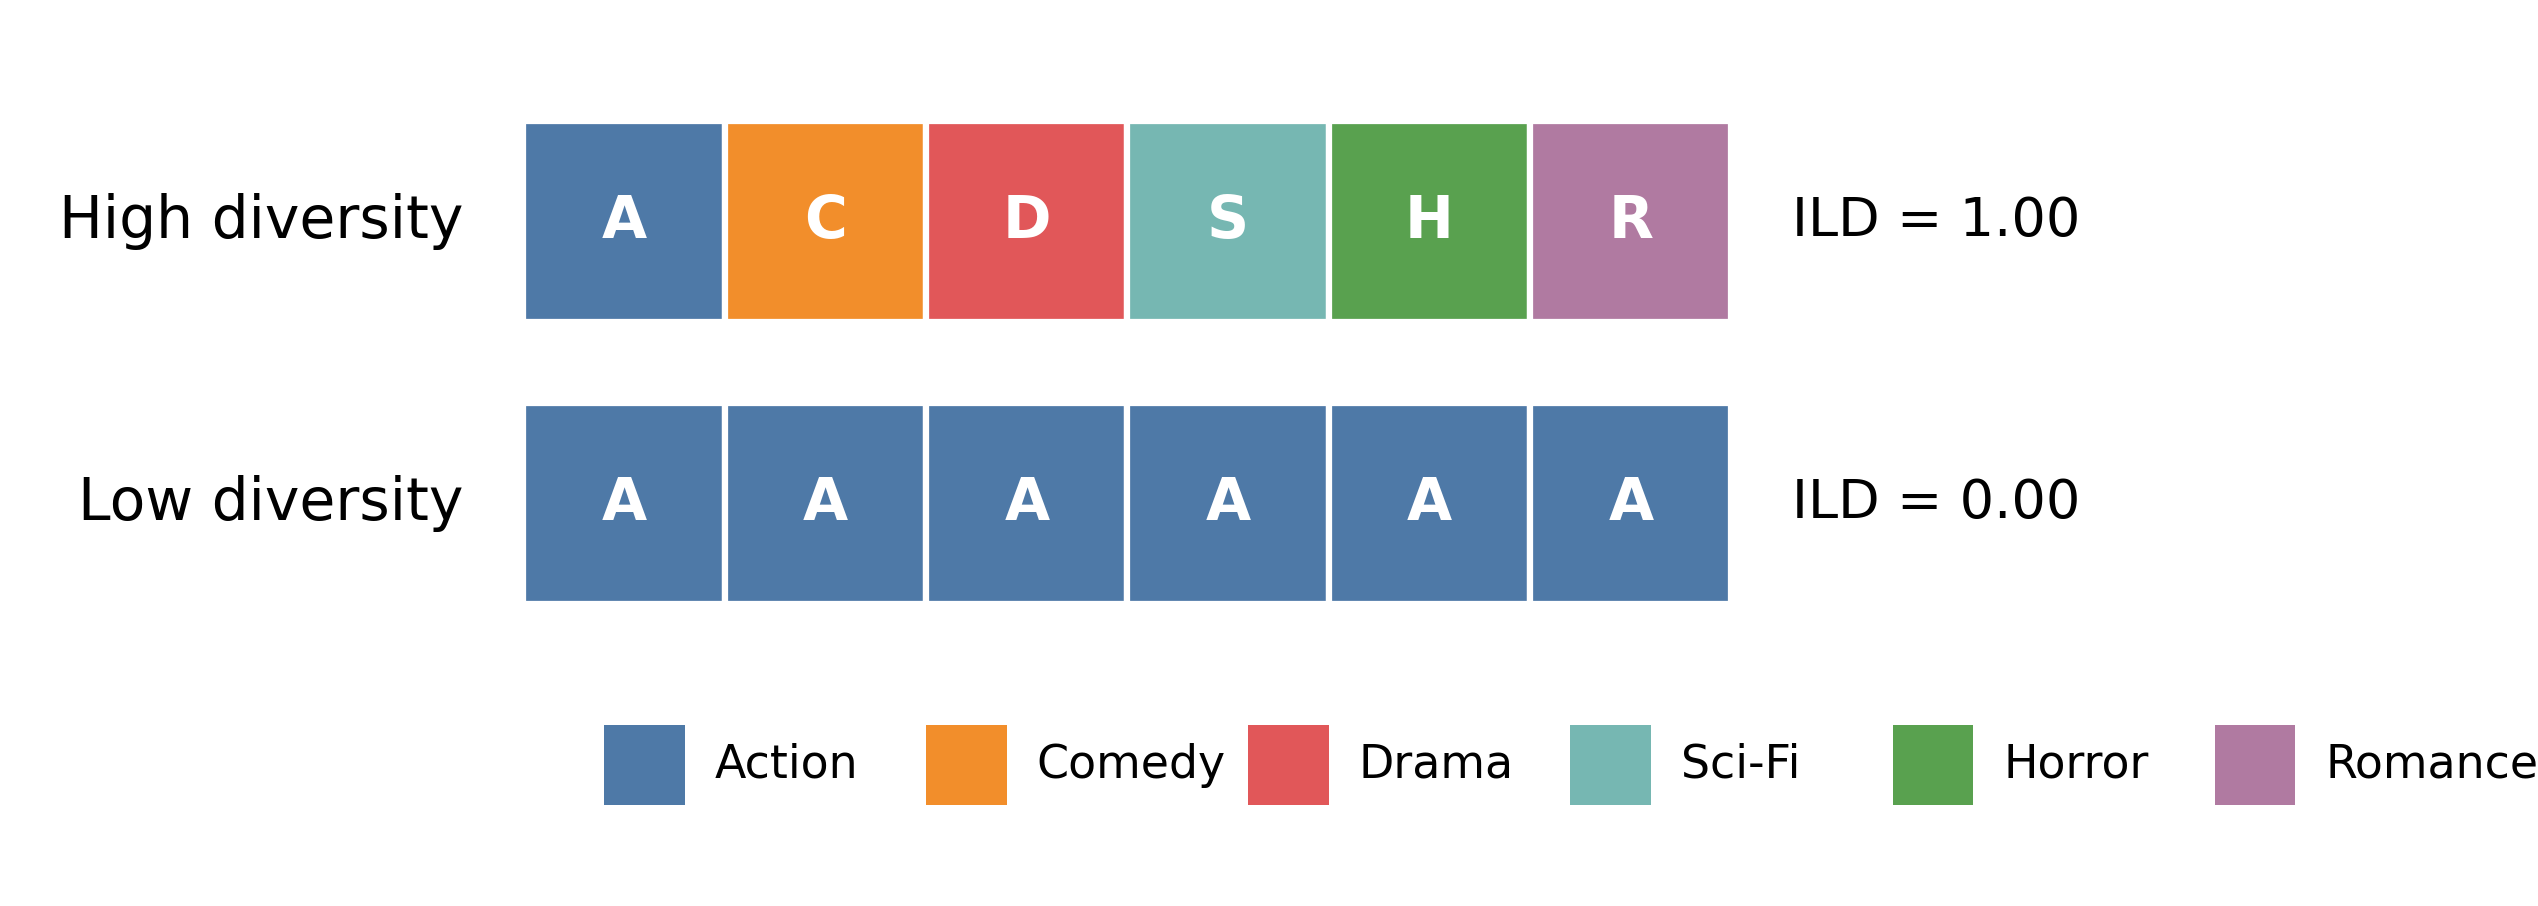
\includegraphics[width=\textwidth]{figures/Diversity_comparison.png}
\end{figure*}

\textbf{Figure.} High diversity (left) spreads recommendations across multiple genres. Low diversity (right) concentrates all recommendations in a single genre.

\orangebox{Did you know that...}
{Intra-List Diversity (ILD) is the most common formulation of diversity in recommender systems. The choice of dissimilarity function $d(i,j)$
is crucial — common options include 1 minus cosine similarity of item feature vectors, or genre/category distance.}

\textbf{Other related metrics}

Diversity measures how different items are from each other, while Novelty measures how new items are to the user.
Serendipity combines both relevance and unexpectedness. Coverage measures catalog utilization.

% ---------- Novelty ----------
\clearpage
\thispagestyle{rankingstyle}
\section{Novelty}
\subsection{Novelty}

Novelty is a ranking metric in recommender systems that measures how unfamiliar or unexpected the recommended items are to
the user. A high Novelty score indicates that the system is suggesting items that the user has not encountered before,
rather than repeating well-known or frequently recommended content. One way to measure Novelty is the following.

\begin{center}
    \[
        Novelty(i) = 1 - \frac{count(\text{users who got recommended} \: i)}{count(\text{users who have not interacted with} \: i)}
    \]
\end{center}

In the literature we can find other ways to compute Novelty such as: $Novelty(i) = -log_2 \left( \frac{count(\text{users who got recommended } \: i)}{count(\text{users who have not interacted with} \: i)} \right)$
or $Novelty = \frac{1}{|S|} \sum_{i \in S} -log P(i)$ where $P(i)$ represents the popularity of item \( i \)
A higher Novelty score means the recommendations contain less mainstream content, encouraging discovery of new items rather
than reinforcing existing preferences.

\textbf{When to use Novelty?}

Novelty is especially useful in scenarios where exploration and discovery are important. Such as content, e-commerce and
retail platforms where recommending new or niche products rather than just trending or best-selling ones can make a difference.

\coloredboxes{
    \item Encourages exploration. Users are exposed to a broader range of content, which can increase
    engagement and retention.
    \item Supports discovery of niche content. Helps mitigate the popularity bias by promoting lesser-known items.
}
{
    \item Potential Trade-off with relevance. High novelty items might be less relevant if the user has no prior
    interest in them.
    \item Potentially overwhelming for users. If novelty is too high, recommendations may feel random or disconnected.
}


\clearpage
\thispagestyle{customstyle}

\begin{figure*}[ht!]
    \centering
    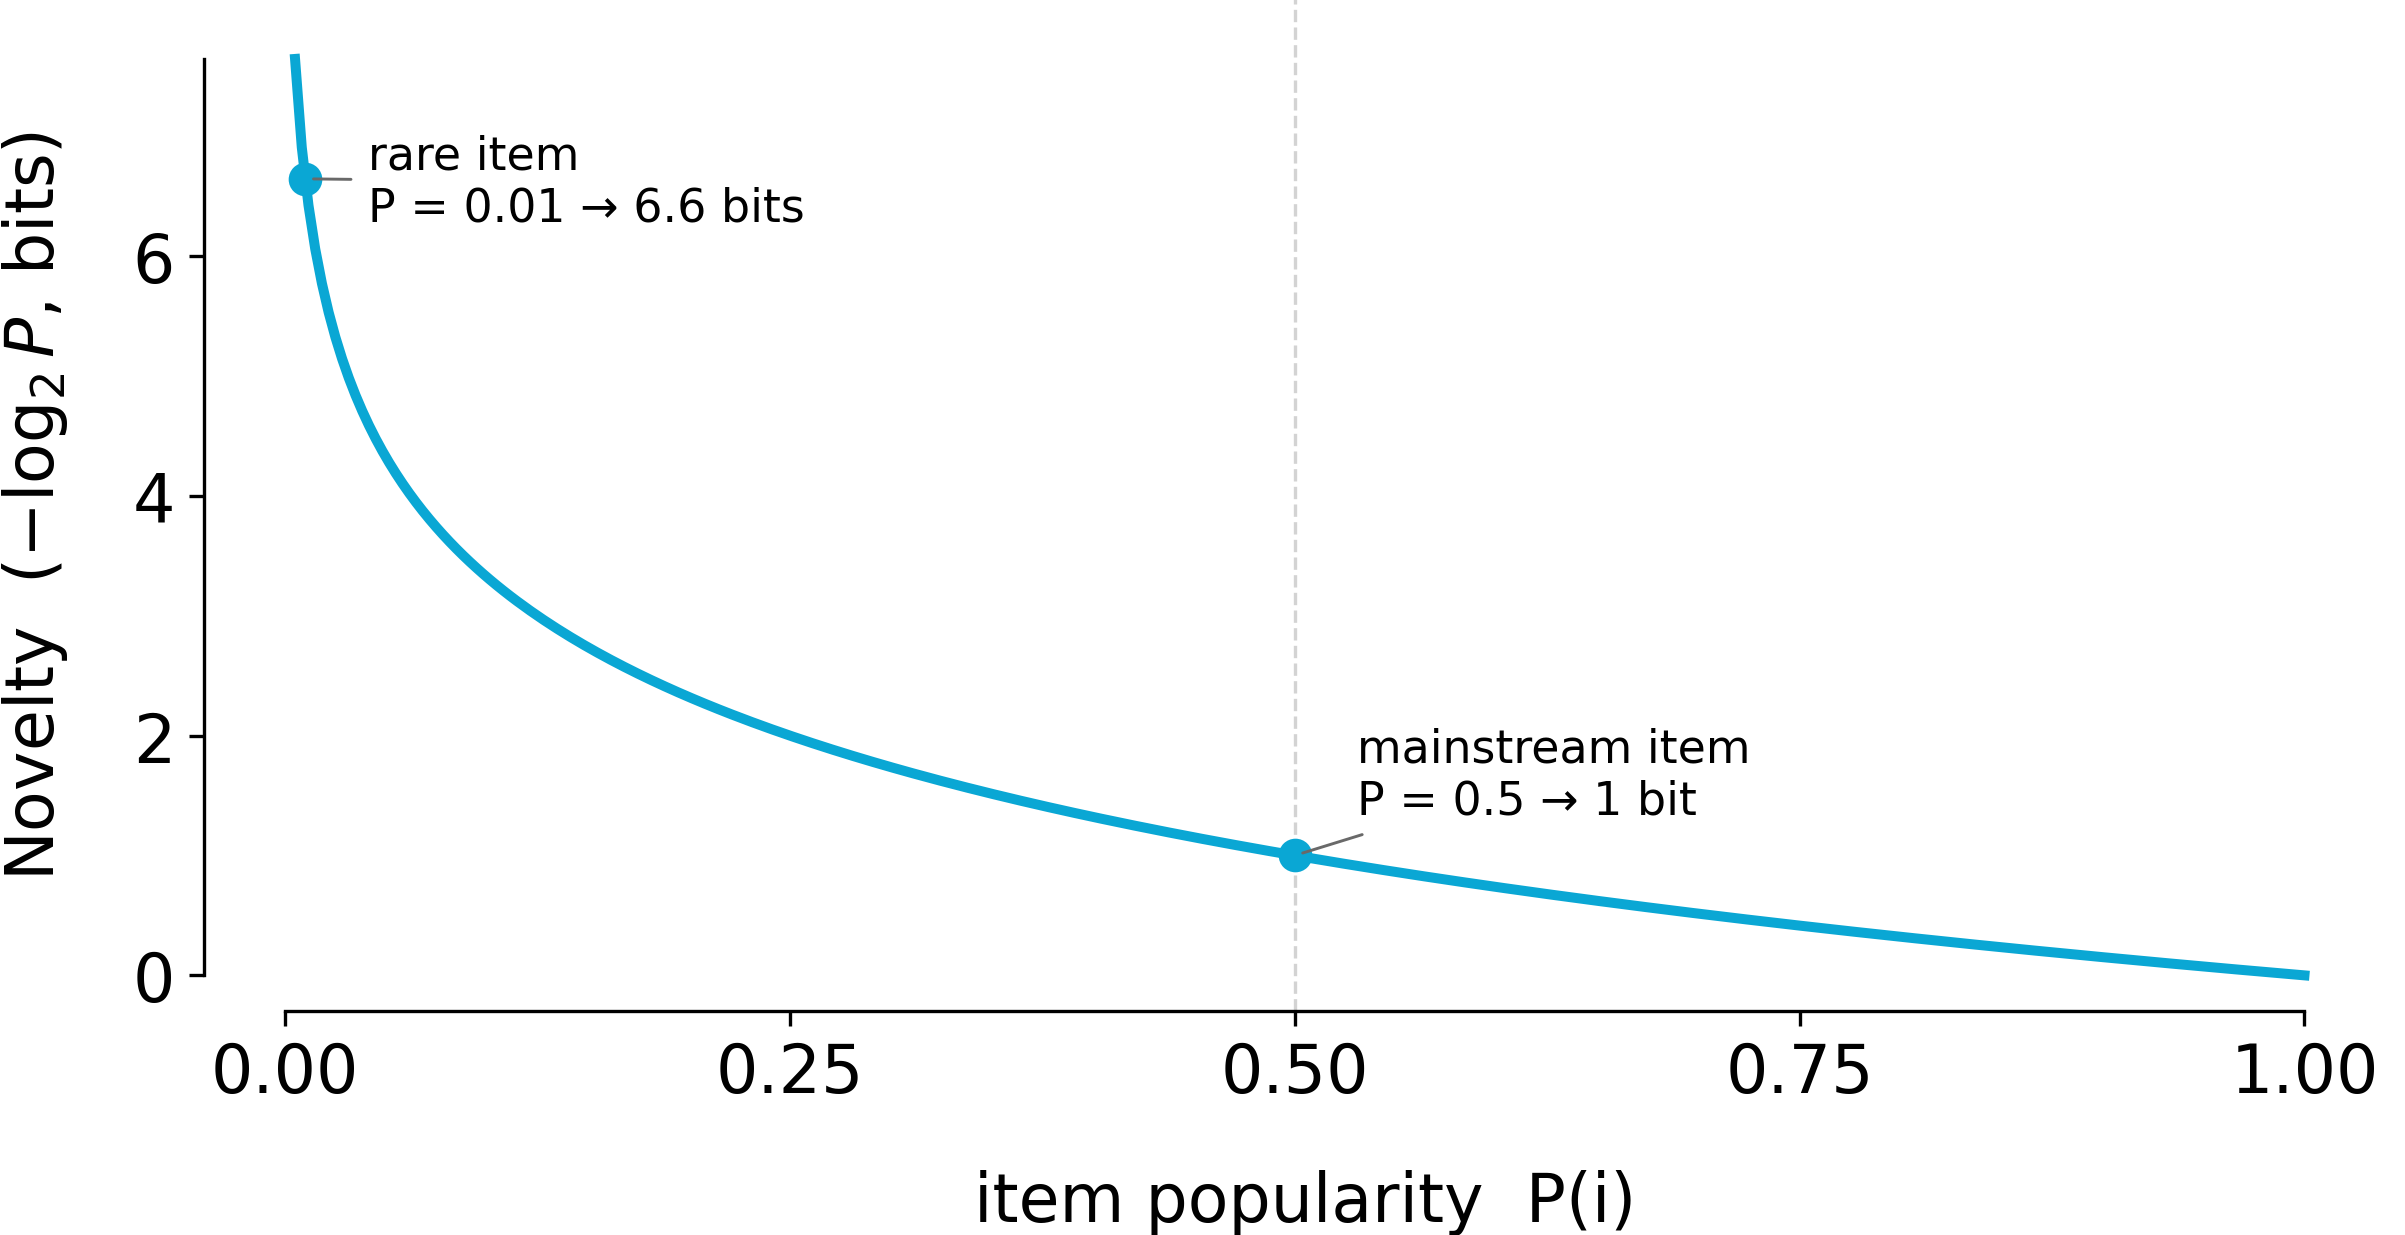
\includegraphics[width=0.6\textwidth]{figures/Novelty_curve.png}
\end{figure*}

\textbf{Figure.} Novelty as a function of item popularity. Rare items (low popularity) have high novelty, while mainstream items have near-zero novelty.

\orangebox{Did you know that...}
{The self-information formulation $Novelty(i) = -\log_2 P(i)$ is borrowed from information theory. A popular item with $P(i) = 0.5$ has novelty of 1 bit,
while a rare item with $P(i) = 0.01$ has novelty of 6.6 bits.}

\textbf{Novelty vs Diversity}

Novelty focuses on how new or unexpected the recommendations are for the user whereas diversity focuses on how different the
recommended items are from each other. Both metrics contribute to exploration but in different ways — novelty ensures
fresh discoveries, while diversity prevents redundancy.

\textbf{Other related metrics}

Novelty is complementary to Diversity and Serendipity. For measuring catalog utilization, see Coverage.
For accuracy-focused ranking evaluation, use nDCG or MAP.

% ---------- Serendipity ----------
\clearpage
\thispagestyle{rankingstyle}
\section{Serendipity}
\subsection{Serendipity}

Serendipity is a ranking and recommendation system metric that measures the extent to which a recommendation is both
relevant and surprising to a user. Unlike conventional accuracy-based metrics, which focus on predicting user preferences
based on past behavior, serendipity evaluates how well a system introduces users to novel and unexpected items they would
not have easily discovered themselves.

\begin{center}
    \tikz{
        \node[inner sep=2pt, font=\Large] (a) {
            {
                $\displaystyle
                Serendipity = \frac{1}{{\color{nmlred}N}} \sum_{i=1}^{N} {\color{nmlcyan}rel(i)} \cdot {\color{nmlpurple}unexp(i)}
                $
            }
        };
        \draw[overlay,-latex,nmlred, semithick] ($(a.south)+(-1.0,0.2)$) to[bend left=15] node[pos=1, left] {number of items} +(-1,-.5);
        \draw[overlay,-latex,nmlcyan, semithick] ($(a.north)+(1.5,-0.1)$) to[bend right=15] node[pos=1, left] {relevance} +(-1,.5);
        \draw[overlay,-latex,nmlpurple, semithick] ($(a.north)+(3.0,-0.1)$) to[bend left=15] node[pos=1, right] {unexpectedness} +(1,.5);
    }
\end{center}

A high serendipity score means the system provides relevant and pleasantly surprising recommendations, while a low score
indicates predictable suggestions.

\textbf{When to use Serendipity?}

Use serendipity when designing recommender systems that aim to provide diverse and engaging recommendations beyond what
users already know. It is particularly useful in domains like music streaming and movie recommendations, where user
satisfaction improves when they encounter unexpected but enjoyable suggestions.

\coloredboxes{
    \item Encourages discovery: Helps users explore new items they wouldn't typically encounter.
    \item Improves long-term engagement. By avoiding repetitive recommendations, it keeps users engaged with the platform.
}
{
    \item Hard to quantify "unexpectedness".
    \item Trade-off with accuracy. Maximizing serendipity may reduce traditional accuracy metrics.
}

\clearpage
\thispagestyle{customstyle}

\begin{figure*}[ht!]
    \centering
    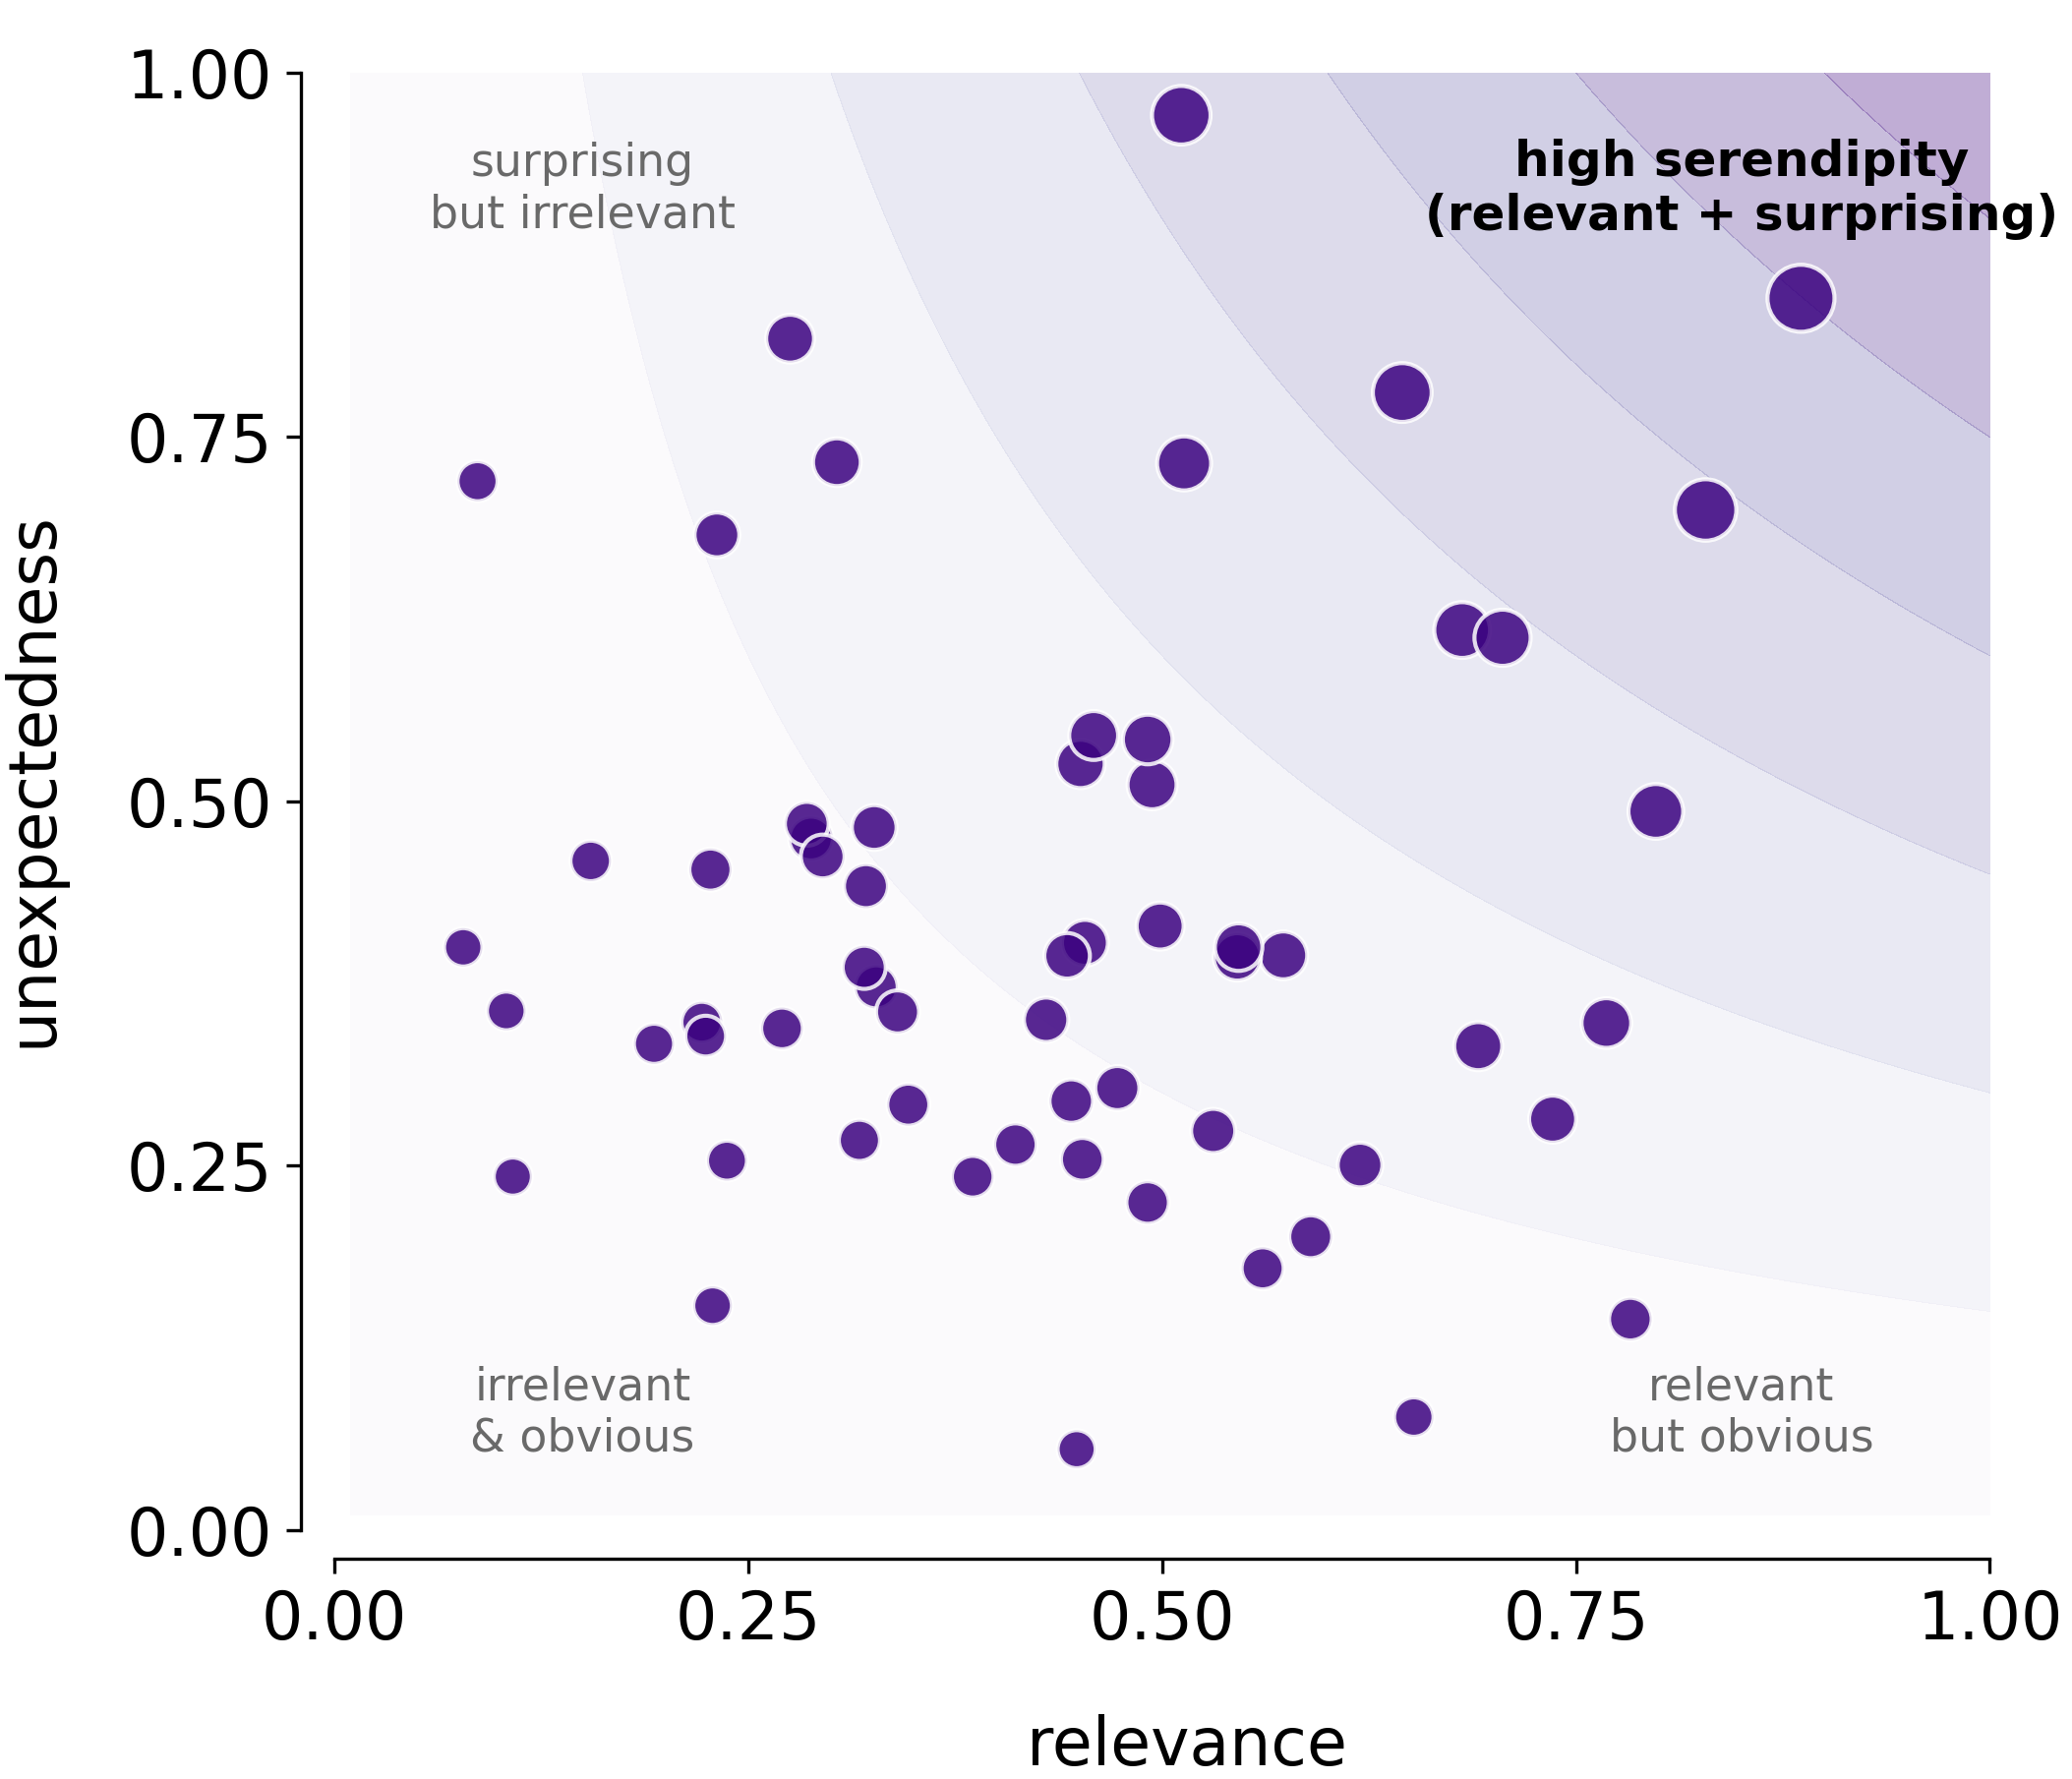
\includegraphics[width=0.6\textwidth]{figures/Serendipity_scatter.png}
\end{figure*}

\textbf{Figure.} Each point is a recommended item. Serendipity is highest (dark) when items are both relevant AND unexpected. The upper-right quadrant represents the ideal serendipitous recommendations.

\orangebox{Did you know that...}
{The term serendipity comes from the 1754 fairy tale "The Three Princes of Serendip." In recommender systems, it captures the idea of
a "happy accident" — finding something valuable that you weren't looking for.}

\textbf{Other related metrics}

Serendipity combines relevance (like Precision) with unexpectedness (like Novelty). For measuring variety without
considering relevance, use Diversity. For catalog breadth, see Coverage.

% ---------- Coverage ----------
\clearpage
\thispagestyle{rankingstyle}
\section{Coverage}
\subsection{Coverage}

Coverage measures how well a recommender system utilizes the full range of available items. It reflects the proportion of
the item catalog that is being recommended to users, ensuring that recommendations are not overly concentrated on a small
subset of popular items. 

\begin{center}
    \tikz{
        \node[inner sep=2pt, font=\Large] (a) {
            {
                $\displaystyle
                Coverage = \frac{|{\color{nmlcyan}\text{recommended items}}|}{|{\color{nmlpurple}\text{total catalog}}|}
                $
            }
        };
        \draw[overlay,-latex,nmlcyan, semithick] ($(a.north)+(0.5,-0.1)$) to[bend right=15] node[pos=1, left] {unique recommended} +(-1,.5);
        \draw[overlay,-latex,nmlpurple, semithick] ($(a.south)+(1.0,0.3)$) to[bend left=15] node[pos=1, left] {total catalog items} +(-1,-.5);
    }
\end{center}

Higher coverage indicates a broader, more diverse recommendation set, while lower coverage suggests a system that primarily
focuses on frequently chosen or trending items.

\textbf{When to use Coverage?}

Use coverage when evaluating how well a recommender system distributes recommendations across the entire catalog. 
It is particularly useful for platforms where content discovery is a priority. If a system recommends only a small fraction
of the available items, users may miss out on relevant but less popular choices.

\coloredboxes{
    \item Reduces popularity bias. Encourages recommendations beyond just the most popular or frequently interacted items.
    \item Enhances user discovery. Helps users explore content they may not have found otherwise.
}
{
    \item Can reduce recommendation accuracy. Expanding recommendations too broadly may lead to less relevant suggestions.
}

\clearpage
\thispagestyle{customstyle}

\begin{figure*}[ht!]
    \centering
    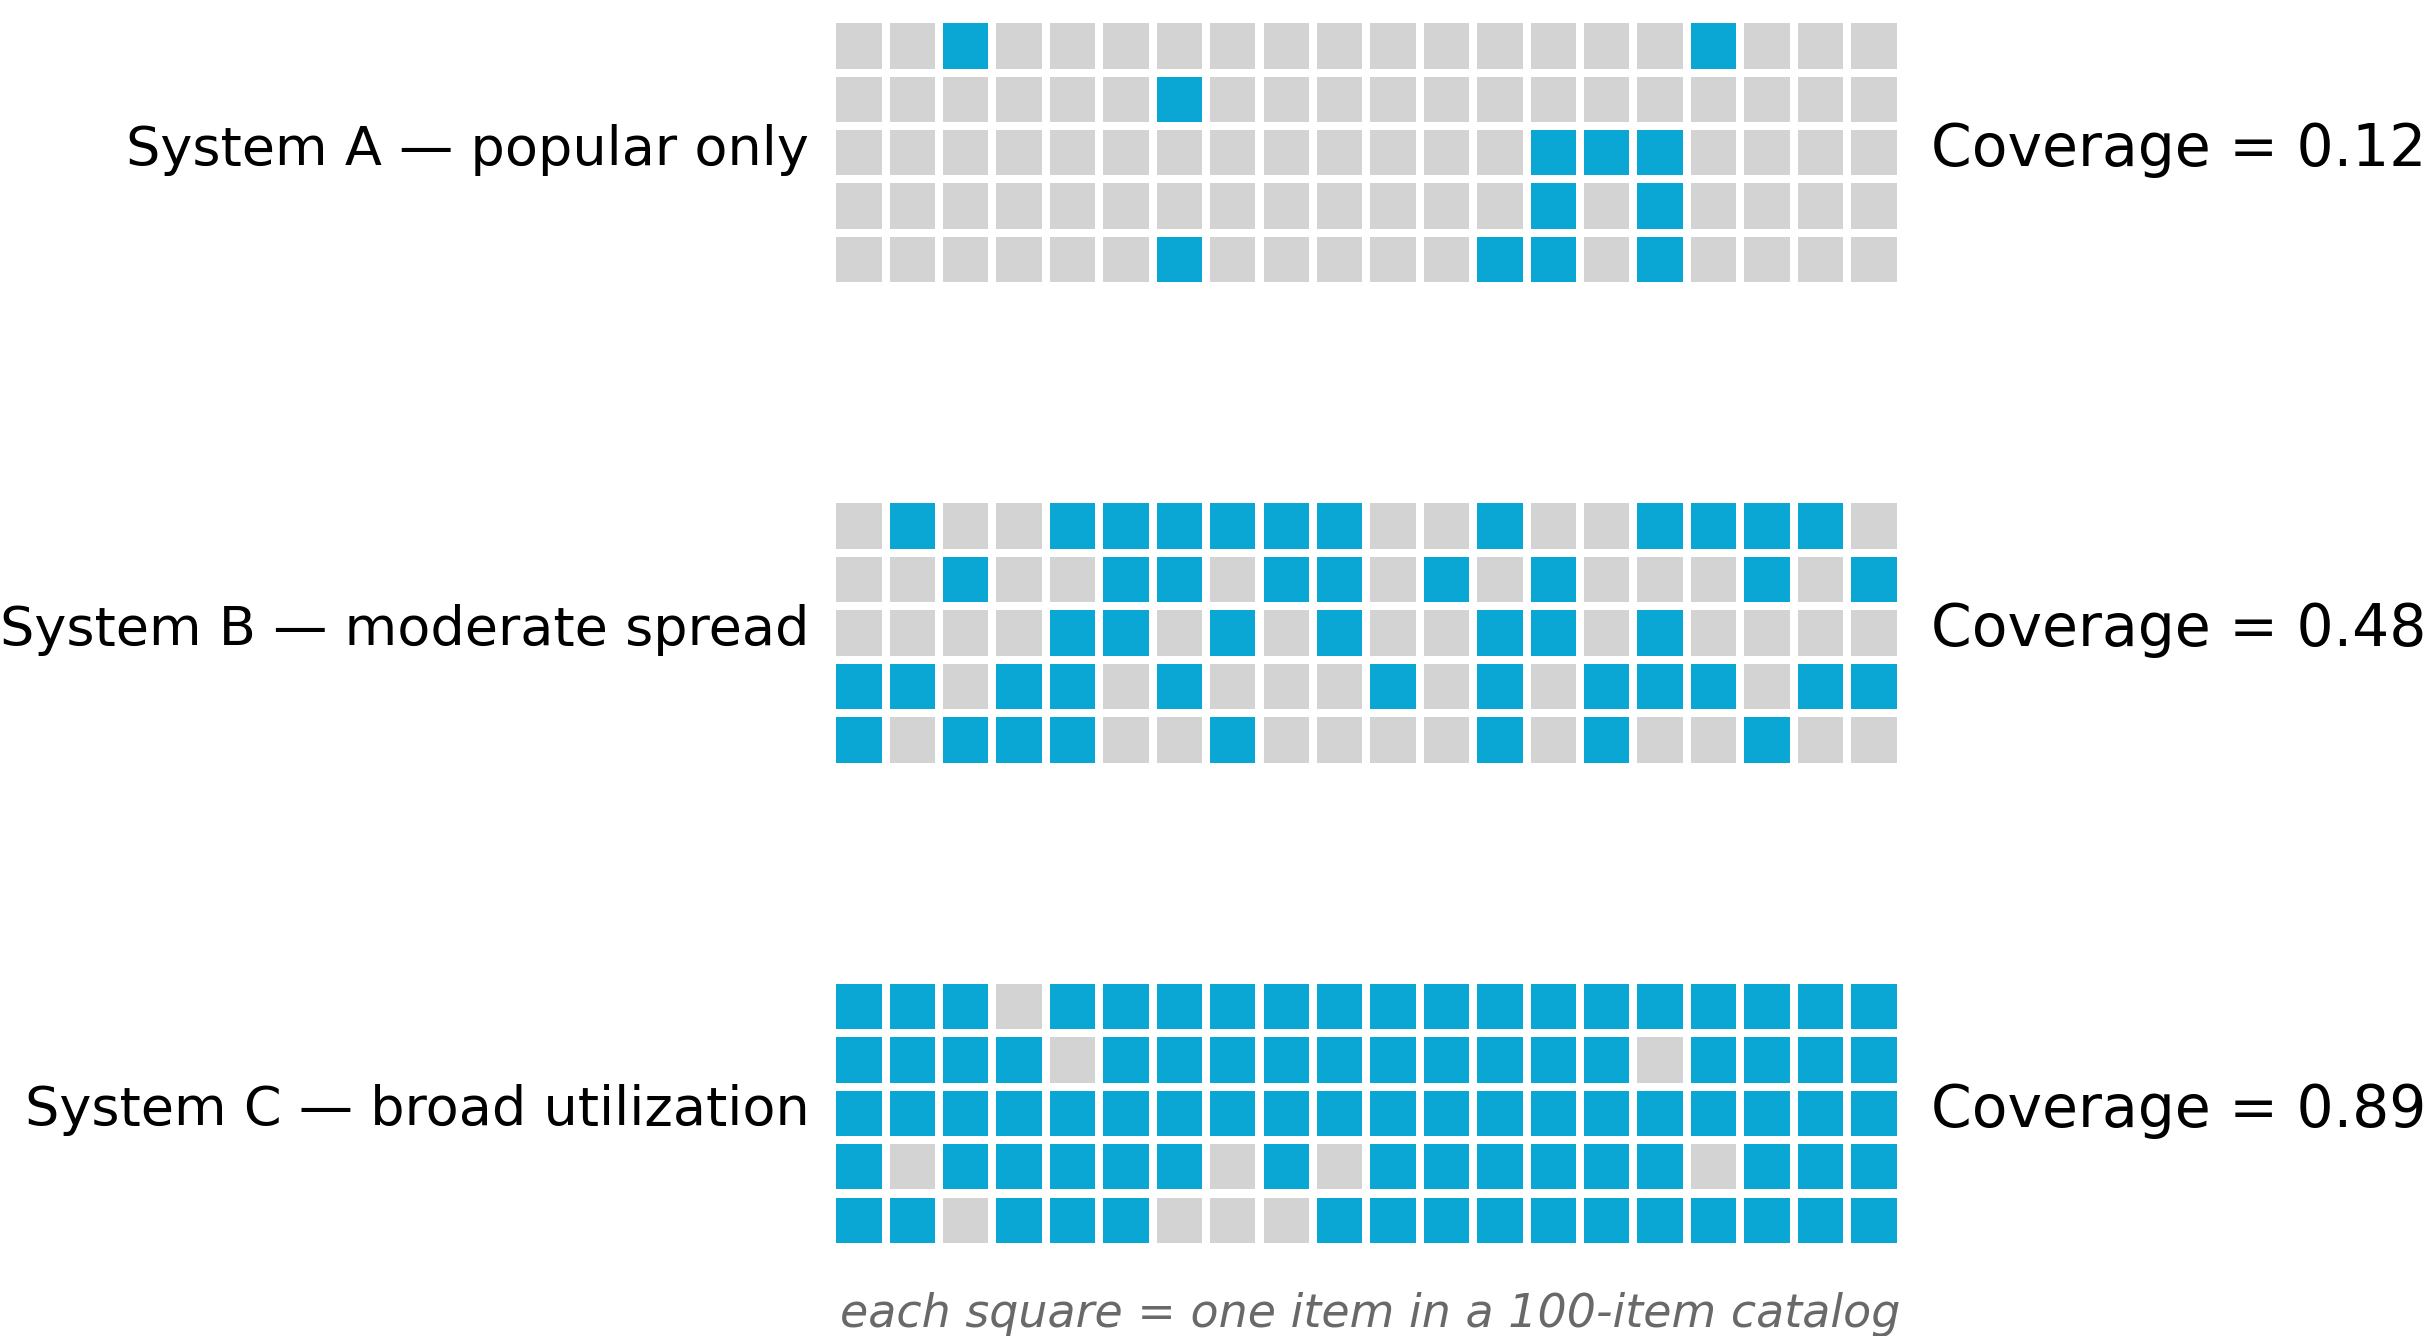
\includegraphics[width=0.6\textwidth]{figures/Coverage_comparison.png}
\end{figure*}

\textbf{Figure.} Three recommender systems with different coverage levels. System A only recommends popular items (12\% of catalog), while System C utilizes 89\% of the full catalog.

\orangebox{Did you know that...}
{Low coverage is a symptom of the "popularity bias" problem. Some recommender systems end up recommending the same small set of popular items
to all users, leaving the long tail of the catalog unexplored.}

\textbf{Other related metrics}

Coverage measures catalog breadth, while Diversity measures within-list variety. For measuring how new items are to individual users, see Novelty.
For accuracy-focused evaluation, use nDCG or MAP.